% This is samplepaper.tex, a sample chapter demonstrating the
% LLNCS macro package for Springer Computer Science proceedings;
% Version 2.20 of 2017/10/04
%
\documentclass[runningheads]{llncs} %
\usepackage{graphicx} % Used for displaying a sample figure. If possible, figure
% files should
% be included in EPS format.
%
% If you use the hyperref package, please uncomment the following line
% to display URLs in blue roman font according to Springer's eBook style:
% \renewcommand\UrlFont{\color{blue}\rmfamily}

\usepackage[utf8]{inputenc}
%%\usepackage{amsmath}
%%\usepackage{amsthm}
\usepackage{amssymb}
\usepackage{threeparttable}
\usepackage{graphicx}
\usepackage{color}
\usepackage{paralist}
\usepackage{framed}
%%\usepackage{caption}
\usepackage{subcaption}
\usepackage{todonotes}
%%\newtheorem{theorem}{Theorem}
%%\newtheorem{corollary}{Corollary}[theorem]
%%\newtheorem{lemma}[theorem]{Lemma}
%%
%%\newtheorem*{example}{Example}
%%\newtheorem{remark}{Remark}

\usepackage[shortlabels]{enumitem}



\usepackage{algorithmic}
\usepackage[ruled,vlined]{algorithm2e}
\usepackage[cmex10,fleqn]{amsmath}
\usepackage{amsfonts}


\newcommand{\hp}{{\sc HeteroPrio}\xspace}
\SetKw{continue}{continue}


%%\pagenumbering{gobble}

\begin{document} %
	%	\title{Contribution Title\thanks{Supported by organization x.}}
%%	\title{Order of Data Transfers between CPU and GPU: A Case Study}
	\title{Performance Models for Data Transfers: A Case Study with Molecular Chemistry Kernels}
	%\titlerunning{Abbreviated paper title}
	% If the paper title is too long for the running head, you can set
	% an abbreviated paper title here
	%
	\author{}
%%%%	\author{First Author\inst{1}\orcidID{0000-1111-2222-3333} \and Second
%%%%		Author\inst{2,3}\orcidID{1111-2222-3333-4444} \and Third
%%%%		Author\inst{3}\orcidID{2222--3333-4444-5555}} %
%%%%	\authorrunning{F. Author et al.} % First names are abbreviated in the running
	% head.
	% If there are more than two authors, 'et al.' is used.
	%
	\institute{Princeton University, Princeton NJ 08544, USA \and Springer
		Heidelberg, Tiergartenstr. 17, 69121 Heidelberg, Germany
		\email{lncs@springer.com}\\
		\url{http://www.springer.com/gp/computer-science/lncs} \and ABC Institute,
		Rupert-Karls-University Heidelberg, Heidelberg, Germany\\
		\email{\{abc,lncs\}@uni-heidelberg.de}} %
	\maketitle              % typeset the header of the contribution
	%
	\begin{abstract} 
%%		
%%		The abstract should briefly summarize the contents of the
%%		paper in 150--250 words.

With increasing complexity of hardwares, systems with different memory nodes are ubiquitous in high performance computing (HPC). It is paramount to develop strategies to overlap the data transfers between memory nodes with the computation in order to exploit the full potential of these systems. In this article, we consider the problem of deciding the  order of data transfers between two memory nodes for a set of independent tasks  with the objective to minimize the makespan. We propose an optimal heuristic to obtain the order of data transfers when there is not any restriction on memory limit. We also show that with finite memory capacity obtaining the optimal order of data transfers is an NP-complete problem. We propose several heuristics for this problem and provide analysis of them on traces obtained by running 3 molecular chemistry kernels, namely, Hartree–Fock , Cholesky contraction, and CCSD on 16 nodes of an HPC system. Our results show that some of our heuristics achieve \% overlap for intermediate memory capacities and are very close to the lower bound of makespan.
		\begin{itemize}
			\item Task-based systems
%%			\item goal is to provide analysis of different scheduling strategies
%%			\item Problem with simple assumption is NP-hard
%%			\item compare with the lower bound of performance
		\end{itemize}
		\keywords{Communication Scheduling  \and Memory Nodes \and Molecular Chemistry.}
	\end{abstract} %
	%
	%
	
	\section{Introduction} 
	
	
%%	\begin{itemize}
%%%%		\item limitation of previous approaches
%%%%		\item scheduling problems are NP-complete, several  phenomena are added to inherent NP-hard optimization problems
%%%%		\item hard to precisely predict the performance of both computations and communications
%%%%		\item number of architectures have increased drastically in recent years
%%%%		\item Task based runtime systems
%%%%		\item Communication is one of the main bottleneck on hpc systems (cite Gullium Aupy work)
%%%%		\item Stress on communication avoidance algorithms (Communication avoidance algorithm)
%%%%		\item A lot of work on the computation scheduling
%%%%		\item Assume communications can be completely overlapped for dense linear algebra computations (Our citations)
%%%%		\item Our framework can be easily extended to any system which operates on different types of memory
%%%%		\item To think what are the bottlenecks, which would restrict us from parallel communications
%%%%		\item Focus and contributions of this paper
%%				
%%	\end{itemize}
		
	With the advent of multicore, and the use of accelerators, it is notoriously cumbersome to exploit the full capacity of a machine. Indeed, there are several challenges come into picture. First, every architecture provides its own efficacy and interface. Therefore, a steep learning curve is required for programmers to take good utilization of all resources. Second, scheduling is a well known NP-Complete optimization problem, and hybrid and distributed resources make this problem harder (we refer ~\cite{webpagescheduling} for a survey on the complexity of scheduling problems and ~\cite{bleuse2015scheduling} for a recent survey in the case of hybrid nodes). Third, due to shared buses, parallel resources, it is hard to obtain a precise model based on prediction of computation and communication timings. Fourth, number of architectures has increased drastically in recent years, therefore it is almost impossible to develop hand tune optimized code for all these architectures. All these observations led to the development of different task based runtime systems. Among several runtimes, we may cite QUARK~\cite{YarKhan:2011:Quark:Manual} and PaRSEC~\cite{parsec} from from ICL, Univ. of Tennessee Knoxville (USA), StarPU~\cite{starpu} form INRIA Bordeaux (FRANCE), Legion~\cite{legion12} from Stanford Univ. (USA), StarSs~\cite{ompss} from Barcelona Supercomputing Center (Spain), KAPPI~\cite{kaapi} from INRIA Grenoble (France). All these runtime systems allow programmers to express their algorithms at the abstract level in the form of direct acyclic graphs, where vertices represent computations and edges represent dependencies among them. Sometimes some static information such as distance to exit (last) node as a priority or affinity of computation towards resources is also provided along with the DAG. Then runtime manages scheduling of computations and communications, data transfer among different memories, computation-communication overlap, load balance in the best possible way.  
		
		
%%	Historically there is a great focus on the design of parallel algorithms and to minimize the complexity of the computations. Also In the last decade, there is a drastic improvement in the hardware to provide perminent rate of computation, but little improvement has been achieved for the rate of data movement. With extreme scale computing, supercomputers face bottlenecks due to ever growing need of data. Therefore focus of HPC community is now changing towards avoiding, hiding and minimizing communications. (Kyelick work and http://science.energy.gov/~/media/ascr/ ascac/pdf/meetings/20140210/Top10reportFEB14.pdf )


	 In the last few decades, there is a drastic improvement in the hardware to provide perminent rate of computation, but little improvement has been achieved for the rate of data movement. With extreme scale computing, supercomputers face bottlenecks due to the need of large amount of data~\cite{ascaccommitteereport2014,yelick2016}. Therefore focus of HPC community is now changing towards avoiding, hiding and minimizing communication costs.
	 
	
	Certain applications such as dense linear algebra kernels have regular structure. Therefore it is possible to associate priorities, based on the task graph structure, with computations, which runtime uses to make the execution efficient. In some applications, such as sparse linear algebra kernels, where programmers do not know the precise structure of the tasks graphs in advance,  tasks are added recursively based on certain sentinel constraints. For such applications, runtime sees a set of independent ready tasks and schedule them on different processing units. It is extremely important for runtimes to decide the order of data transfers for these scheduled computations such that overlap between computations and communications can be maximised. This is the main topic of this paper. We propose different strategies for runtimes such that it can maximize the overlap of computation and communication for kernels running on two different memory nodes. We prove that one of our proposed strategies is an optimal one when we do not have any restriction on the capacity of memory node. We also prove that order of communication on two memory nodes  with the objective of minimizing the makespan is  NP-Complete. We evaluate our strategies on a cluster of homogeneous nodes. But our approach is generic and easily adaptable to any system which operates on different memory spaces. Here are the important contributions of this paper.
	
	\renewcommand{\labelitemi}{$\bullet$}
	\begin{itemize}
		\item Proposed different scheduling strategies with the objective to minimize the makespan
		\item An optimal strategy and its proof, when there is not any memory capacity constraint on target machine
		\item NP-Completeness proof for the general data-transfer problem  
		\item Linear programming formulation of the problem
		\item Numerous  experiments to assess the effectiveness of our strategies on molecular chemistry kernels 
	\end{itemize}
		


\section{Related Work}



Historically there has been a great emphasis on the development of parallel algorithms and minimizing the complexity of computations. As the number of computation cores has increased drastically in recent years, supercomputers face bottleneck due to communication required by an application. Hence, in recent years the focus has changed towards developing communication avoiding algorithms, strategies to hiding communications and  minimizing the data accessed by applications~\cite{yelick2016}. 

  
The problem of scheduling tasks has been highly studied in literature and this problem is known to be NP-Complete~\cite{GareyJohnson}.  Many static and dynamic strategies have been proposed and analyzed for this problem~\cite{heft-Topcuoglu,hipc16multiresource,ipdps16starpu}. There ia also a number of studies in the direction of task scheduling with the emphasis of improving locality and minimizing the communication cost~\cite{starpu,heft-Topcuoglu}. Stanisic et. al proposed a heuristic to schedule tasks on a computing resource where most of its data is available~\cite{luka-dmdar}. Similar approach has been adopted by Agullo et. al for the scheduling of sparse linear algebra kernels~\cite{agullo_fmm}.  Predari et.al  proposed  heuristics to  partition the task graph across a number of processors such that inter processor communication can be minimized ~\cite{predari:tel-01518956}.

The problem considered in this paper also can be viewed as a flow shop problem. Communication and computation timings of a task can be considered as processing timings on different machines.  Johnson has provided scheduling strategies for 2 and 3-machine flow shop problems with infinite memory case~\cite{johnson}. 2-machine flow shop problem with finite memory capacity has been proven NP-Complete by Papadimitriou et. al~\cite{Papadimitriou:1980:FSL:322203.322213}. The main difference with the our approach is that they consider unit buffer requirement on 1st machine after job completion. On the contrary, our approach is designed for tasks appearing in scientific workloads whose sizes are highly irregular and memory is acquired before starting the communication.

There is also a numerous study pertaining to the scheduling with limited memory and storage, since the work of Sethi and Ulman, register allocation for arithmetic expressions~\cite{Sethi:1970:GOC:321607.321620}.  Sarkar et. al  worked on the scheduling of graphs of smaller-grain tasks with limited memory, where each task requires homogeneous data size ~\cite{vsarkar-pact}. The same work has been extend by Loris et. al for task graphs where memory requirement of each task is highly irregular~\cite{loris-ipdps18}.



\begin{itemize}
	%%	\item Papadimitriou work
	%%	\item Johnson's work
	%%	\item Kethrin Yelik work
	%%	\item Task graph work by Loris
	%%	\item Vivek Sarkar work
	%%	\item Register coloring by Sethi
	\item roofline model
	\item theoretical/performance work on molecular chemistry kernels
\end{itemize}

%%	\begin{itemize} 
%%%%		\item may consider transfer between two memory nodes
%%%%		 \item perform experiments for transfer between CPU and GPU 
%%%%%%		\item Task based approach, communication-computation maximum overlap 
%%%%%%		\item concurrent execution of multiple kernels 
%%%%%%		\item proof for maximum computation-communication overlap with infinite memory 
%%%%%%		\item Problem statement : NP complete problem
%%%%%%		\item extended version of NP complete problem 
%%%%%%		\item Different proposed heuristics for order of data transfers 
%%%%		\item Simulation results for all proposed heuristics 
%%%%%%%		\item Experiments on actual platform with the best proposed heuristic 
%%	\end{itemize}
	\todo[inline]{SKumar: Modify both proofs }
	\section{Data Transfer problem formulation}
	
%%	\newpage 
	\section*{Order of data transfers}
	
	To exploit the full potential of a system tasks may get scheduled on processing
	units where all of their data does not reside. A task may require all of its data
	in local memory before starting the execution. There may be multiple tasks
	scheduled on a processing unit, which require to transfer data from the same
	memory node. Order of data transfers for such tasks is very crucial for the
	communication-computation overlap, thus for the overall performance. Tasks may
	also produce some output data, which, in general, is very less.  It is often the case that future tasks running on the same memory node require output data of the past tasks. Therefore, most runtime systems transfer data to other memory nodes based on the demand -- not immediately. It is possible that all output data can be stored in a preallocated separate buffer on a memory node. Hence, we do not consider output data separately in our analysis and assume that output data is negligible (zero or stored in a separate buffer) for each task. We prove that order of execution of such tasks with finite memory capacity, is an NP-complete problem.
	
	
	\subsection{Infinite Memory Case}
	Let $S$ be the set of tasks assigned on processor $P$ with memory unit $M$, and this set of tasks  need input data from another memory unit $M'$. We assume that size of $M$ is very large and there will not be any memory capacity restriction for tasks.
	
	
	\begin{algorithm}
	\caption{\label{alg:OrderOfExecutionInfinteMemory}Algorithm to determine the order of processing for a set of ready tasks (infinite memory case)}
	\begin{algorithmic}[1]
		\STATE Divide ready tasks in two sets $S_1$ and $S_2$. If computation time of a task $T$is not less than its communication time, then $T$ is in $S_1$ otherwise $S_2$.
		\STATE Sort $S_1$ in queue $Q_1$ by non-decreasing communication times
		\STATE Sort $S_2$ in queue $Q_2$ by non-increasing computation times
		\WHILE{all tasks did not complete}
		\IF{$Q_1 \neq \emptyset$}
		\STATE remove a task $T$ from beginning of $Q_1$ for processing
		\ELSE 
		\STATE remove a task $T$ from beginning of $Q_2$ for processing
		\ENDIF
		\ENDWHILE
	\end{algorithmic}
\end{algorithm}
	
	
	\noindent \textbf{Claim} : Order provided by Algorithms~\ref{alg:OrderOfExecutionInfinteMemory} achives the optimal makespan for a set of ready tasks.
	
	\begin{proof}
		Let us first define some notations which we need for this proof.
%%		\todo[inline]{SKumar: Specify the destination for all notations}
		\begin{align*}
		t : & \text{Time at which data transfer for task A started in original schedule}\\
		S_A : & \text{ Start of computation  time of task A in original schedule}\\
		S_B : & \text{ Start of computation time of task B in original schedule}\\
		S'_A : & \text{ Start of computation time of task A in swapped schedule}\\
		S'_B : & \text{ Start of computation time of task B in swapped schedule}\\
		CM(A) : & \text{ Data transfer time for task A}\\
		CM(B) : & \text{ Data transfer time for task B}\\
		CP(A) : & \text{ Computation time of of task A}\\
		CP(B) : & \text{ Computation time of task B}\\
		\rho : & \text{ ratio of length of task and data transfer time}
		\end{align*}
	\end{proof}
	
	Let $S$ be the schedule obtained by the above heuristic and $O$ be an optimal schedule. We prove the above claim by converting $S$ to $O$ and showing that at each step completing time of intermediate schedule is not less than the completion time of original schedule $S$. In order to do so, we make sure order of two tasks in both schedules $S$ and $O$ is same. If not, We perform swapping of two tasks.
	
	\noindent If we prove the swapping strategy for two contiguous tasks holds, then the same strategy transitively hold for any two tasks of Schedule $S$ 
	
	
	Let $A$ and $B$ are two contiguous tasks of schedule $S$, which need to be swapped.
	\todo[inline]{SKumar: draw an equivalent xfig diagram}
	\begin{figure}[htb]
		\centering
		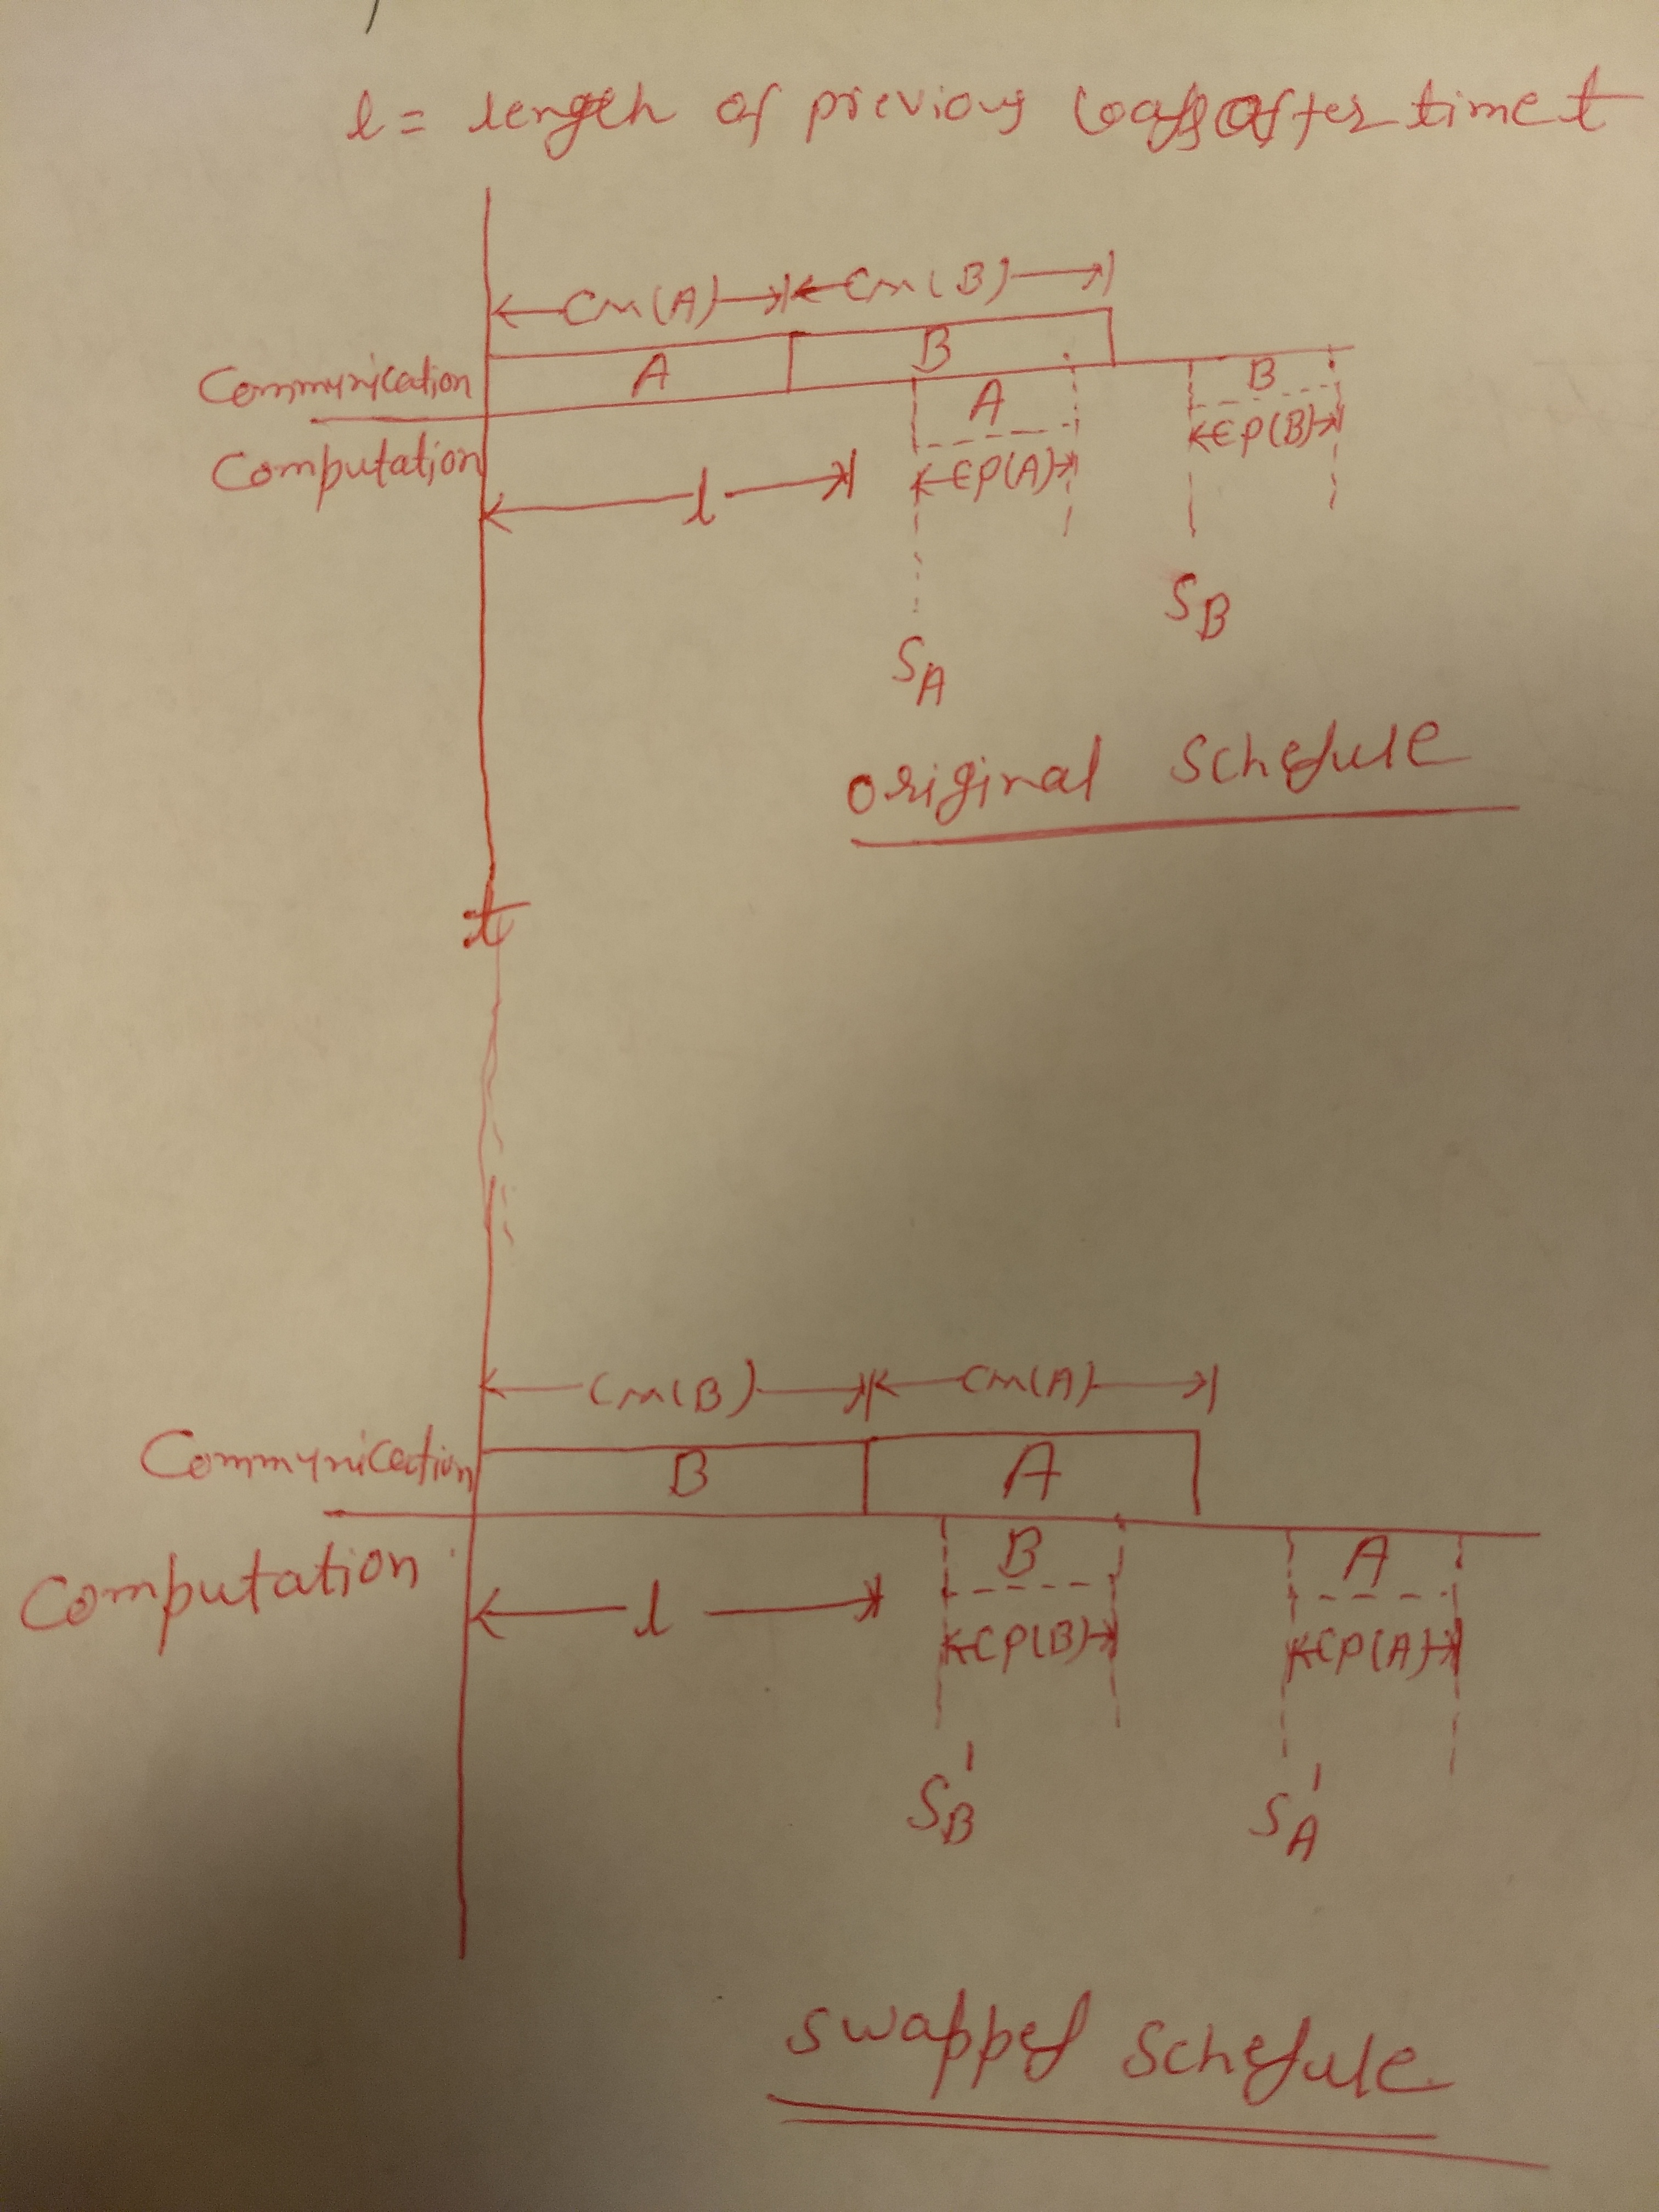
\includegraphics[width=\textwidth, height=0.5\textheight, 
		keepaspectratio]{Figs/swappedSchedule.jpg}
		\caption{ \label{fig:bothSchedule} Original and Swapped Schedule}
	\end{figure}
	
	We can write the following constraints based on the two schedules of the Fig~\ref{fig:bothSchedule}.
	
	\begin{eqnarray*}
		S_A & = & max(CM(A), l) \\
		S_B & = & max(S_A + CP(A), CM(A) + CM(B))
	\end{eqnarray*}
	
	Completion time in original Schedule = $S_B + CP(B)$
	\begin{eqnarray*}
		S'_B & = & max(CM(B), l) \\
		S'_A & = & max(S'_B + CP(B), CM(A) + CM(B))
	\end{eqnarray*}
	
	Completion time in swapped Schedule = $S'_A + CP(A)$
	
	Our goal is to prove the following inequality.
	\begin{eqnarray*}
		S_B + CP(B) & \le & S'_A + CP(A)
	\end{eqnarray*}
	\begin{proof}
		\begin{eqnarray*}
			S_B + CP(B) & = & max(S_A + CP(A)+CP(B), CM(A) + CM(B) + CP(B))\\
			& = & max(CM(A) + CP(A) + CP(B), l+CP(A) + CP(B), CM(A) + CM(B) + CP(B)) 
		\end{eqnarray*}
		Case I: $A, B\in ST_1, CM(A) \le CM(B), CP(A) \ge CM(A), CP(B) \ge CM(B)$
		\begin{eqnarray*}
			S_B + CP(B) & = & max(CM(A) + CP(A) + CP(B), l+CP(A) + CP(B), CM(A) + CM(B) + CP(B)) \\
			& \le & max(CM(A) + CP(B), l+CP(B), CM(B)+CP(B)) + CP(A)\\
			& = & max(CM(B) + CP(B), l + CP(B)) + CP(A) \\
			& = & max(max(CM(B), l) + CP(B), CM(A) + CM(B)) + CP(A) \\
			& = & max(S'_B + CP(B), CM(A) +CM(B)) + CP(A) \\
			& = & S'_A + CP(A)
		\end{eqnarray*}
		Case II: $A, B\in ST_2, CP(A) \ge CP(B), CP(A) < CM(A), CP(B) < CM(B)$
		\begin{eqnarray*}
			S_B + CP(B) & = & max(CM(A) + CP(A) + CP(B), l+CP(A) + CP(B), CM(A) + CM(B) + CP(B)) \\
			& \le & max(CM(A) + CP(B), l+CP(B), CM(A)+CM(B)) + CP(A)\\
			& = & max(CM(A) + CM(B), l + CP(B)) + CP(A) \\
			& = & max(CM(B) + CP(B), l + CP(B), CM(A) + CM(B)) + CP(A) \\
			& = & max(max(CM(B), l) + CP(B), CM(A) + CM(B)) + CP(A) \\
			& = & max(S'_B + CP(B), CM(A) +CM(B)) + CP(A) \\
			& = & S'_A + CP(A)
		\end{eqnarray*}
		Case III: $A \in ST_1, B\in ST_2, CP(A) \ge CM(A), CP(B) < CM(B)$
		\begin{eqnarray*}
			S_B + CP(B) & = & max(CM(A) + CP(A) + CP(B), l+CP(A) + CP(B), CM(A) + CM(B) + CP(B)) \\
			& \le & max(CM(A) + CP(B), l + CP(B), CM(B) + CP(B)) + CP(A)\\
			& \le & max(CM(A) + CM(B), l + CP(B), CM(B) + CP(B)) + CP(A) \\
			& = & max(max(CM(B), l) + CP(B), CM(A) + CM(B)) + CP(A) \\
			& = & max(S'_B + CP(B), CM(A) +CM(B)) + CP(A) \\
			& = & S'_A + CP(A)
		\end{eqnarray*}
	\end{proof}	


This problem can be expressed as 2-machine flowshop problem with infinite storage, where communication time is the processing time on first machine and computation time is the processing time on second machine and the goal is to minimize the overall makespan. In [], Johnson's algorithm also achieves the optimal makespan but the proof techniques and algorithm are quite different from ours.
	\subsection{Finite Memory}
	
	In general, order of task execution with input and output data transfers can be 
	viewed as  3-machine flowshop problem, where processing time on 1st machine is 
	input data transfer time,  processing time on 2nd machine is task execution time, 
	processing time on 3rd machine is output data transfer time  and the objective is 
	to minimize the total makespan. This is a well known NP-complete problem. 
	
	
	\noindent\textbf{Probelm  $DT$} : A set of tasks $ST=\{T_1, \cdots, T_n\}$ is scheduled on a processing 
	unit $P$  with memory unit $M$ of capacity $C$. Input data for tasks of $ST$ reside on 
	another memory unit $M'$. $comm_i$ is the time to transfer input data from $M'$ to $M$ for task 
	$T_i$,  $e_i$ is the execution time of task $T_i$ on $P$. We assume that these tasks  do not produce any output data.  Given $L$, is there a feasible schedule $S$ for $ST$ such that makespan of $S$, $\mu(S) \le L$?
%%	What is the order of execution of $ST$ on $P$ such that 
%%	makespan of	$ST$ is minimal? 
%%	
	\begin{theorem}
		Problem $DT$ is NP-complete.
	\end{theorem}
   \begin{proof}
   	
   	Proving $DT$ is NP-complete requires first to show that decision version of this problem can be 
   	verified by a polynomial time nondeterministic algorithm, and then showing that a known 
   	NP-complete problem is polynomially reducible to this problem. As usual first job is simple and can 
   	be 
   	done in linear time, given a schedule we can check that at each change point memory capacity is 
   	restricted and a task starts execution only after its input data is transferred to $M$. In our case, the 
   	known NP-complete problem that can be reduced to problem $DT$ is the following.
   	
   	
   	\noindent \textbf{Three Partition Problem (3PAR)} : Given a set of $3m$ integers $A = \{ a_1,  
   	\cdots, a_{3m }\}$, is there a partition of $A$ into $m$ triplets $TR_i = \{a_{i_1}, a_{i_2}, a_{i_3}\}$, 
   	such that $\forall i, a_{i_1} + a_{i_2}  + a_{i_3}  = b$, where $b=(1/m) \sum a_i $?
   	
   	This problem is known to be NP-complete.
   	
   	
   	\noindent Let us first show that $3PAR$ problem reduces in polynomial time to problem $DT$.  
   	Suppose that we 
   	are given an instance  $A = \{ a_1,  \cdots, a_{3m }\}$ of $3PAR$ problem. It is immediately obvious 
   	that $a_i>1$, since we can always add sufficiently large integers to $a_i$'s and scale the problem 
   	accordingly.  This scaling will not affect in any way the existence of a solution for the instance of $3PAR$ problem. Consequently, given any instance of the $3PAR$ problem, we construct an instance $I$ of the problem $DT$ such that $I$ has a schedule with makespan bounded by $L$ iff the instance 
   	$I$ of $3PAR$ problem has a solution. The instance of problem $DT$ will have $4m+1$ tasks.
   	
   		\begin{table*}[htb]
   			\begin{tabular}{ |c|c|c| }
   				\hline
   				Task & Input Transfer time ($comm_i$)& Computation time ($e_i$)\\ \hline
   				$K_0$ & $0$ & $3$ \\ \hline
   				$K_1, \cdots, K_{m-1}$ & $b'=b+3x$ & $3$\\ \hline
   				$K_m$ & $b'=b+3x$ & $0$ \\ \hline
   				$1\le i \le 3m, A_i$ & $1$ & $a_i' = a_i +x$\\ \hline
   			\end{tabular}
   		\end{table*}
   	Where $x= 2 max\{a_i:1\le i\le 3m\}$\\ 
   	Memory capacity $C=b'+3$ and $L=m(b'+3)$, this completes the construction of instance $I$ of the 
   	problem $DT$.
   	
   	$Transfer time = Latency + \frac{Data Volume}{Bandwidth}$, for simplicity we consider Latency=0 
   	and Bandwidth=1, (implies Input data volume = Input transfer time), otherwise we can adjust $C$ in 
   	a way such that at any point in a schedule at max one $K_i$ and three $A_i$ tasks can be active.
   	
   	
   	We show that $I$ has a schedule $S$ with $\mu(S) \le L$ iff the original instance of $3PAR$ 
   	problem  has a solution. Notice that sum of transfer times and sum of computation times, both are 
   	equal to $L$, therefore $\mu(S) \le L$ iff $\mu(S)=L$  and there is no idle time on both channels in 
   	$S$. It indicates that first task is $K_0$ and last task is $K_m$.
%%   	
%%   	\todo[inline]{SK: Unable to argue why only $A_i$ tasks will run on communication channel when 
%%   	$K_0$ is running on computation channel.}
   	
   
   	Now we prove that any feasible schedule of $I$ corresponds to a decomposition of $A$ into m 
   	triplets $TR_i = \{a_{i_1}, a_{i_2}, a_{i_3}\}$ such that $\forall i, a_{i_1} + a_{i_2}  + a_{i_3}  = b$. Every 
   	feasible schedule has to consist of $m$ segments like the one shown in Fig~\ref{fig:firstSegment}. Each segment provides a triplet  $\{a_{i_1}, a_{i_2}, a_{i_3}\} $such that  $a_{i_1} + a_{i_2}  + a_{i_3}  = b$.
   	
	Any schedule $S$ of $I$ having no idle time must start with $K_0$. No other $K_i$ tasks can be active with $K_0$, otherwise we would get idle time on computation channel ($b'>3, b'-2>max\{a_i':1\le i\le 3m\},  \text{and } b'-1 > 2 max\{a_i':1\le i\le 3m\}$). Hence three $A_i$ tasks must follow $K_0$.   	 
   	Memory requirement of other $K_i$ tasks is $b'$ and $2b'>C$, therefore at any point in schedule at max one $K_i$ task can be active. Sum of duration of all $K_i$ tasks = $3 + (m-1)(b'+3) + b' = m (b'+3)=L$, hence at each point in $S$ exactly one $K_i$ task is active. When $K_i$ task is in computation phase, no other $K_i$ tasks can be active in that duration, therefore  $3A_i$ tasks must complete data transfers in that duration. After that next task must be a 
   	$K_i$ task, otherwise total makespan would be more than $\sum(transfertime(k_i))  + 
   	\sum(computetime(k_i)) =L$. When communication for  $K_i$ task starts we exactly have $3A_i$ 
   	tasks whose data is available in local memory. Hence three $A_i$ tasks are scheduled for computation. Now we must prove that $a_{i_1}' + a_{i_2}'  + a_{i_3}'  = b'$.
   	
   	This is true because if $a_{i_1}' + a_{i_2}'  + a_{i_3}'  > b'$, total used memory after the data transfer 
   	for  $K_i$ task finishes is atleast $b'+1$, hence only $A_i$ tasks can be considered, which will lead to a schedule in which at a point only $A_i$ tasks are active on both channels, therefore length of 
   	schedule would be more than $L$, and if $a_{i_1}' + a_{i_2}'  + a_{i_3}'  < b'$, then we have idle time on computation channel.
   	
   	Conversely, if such a partition of $A$ is achievable, then we can construct a feasible schedule $S$ 
   	without idle times by the pattern depicted in Fig~\ref{fig:firstSegment}. We have shown that $3PAR$ 
   	problem reduces to $DT$, and hence problem $DT$ is NP-complete.
   	
   	
   	\begin{figure}[htb]
   		\centering
   		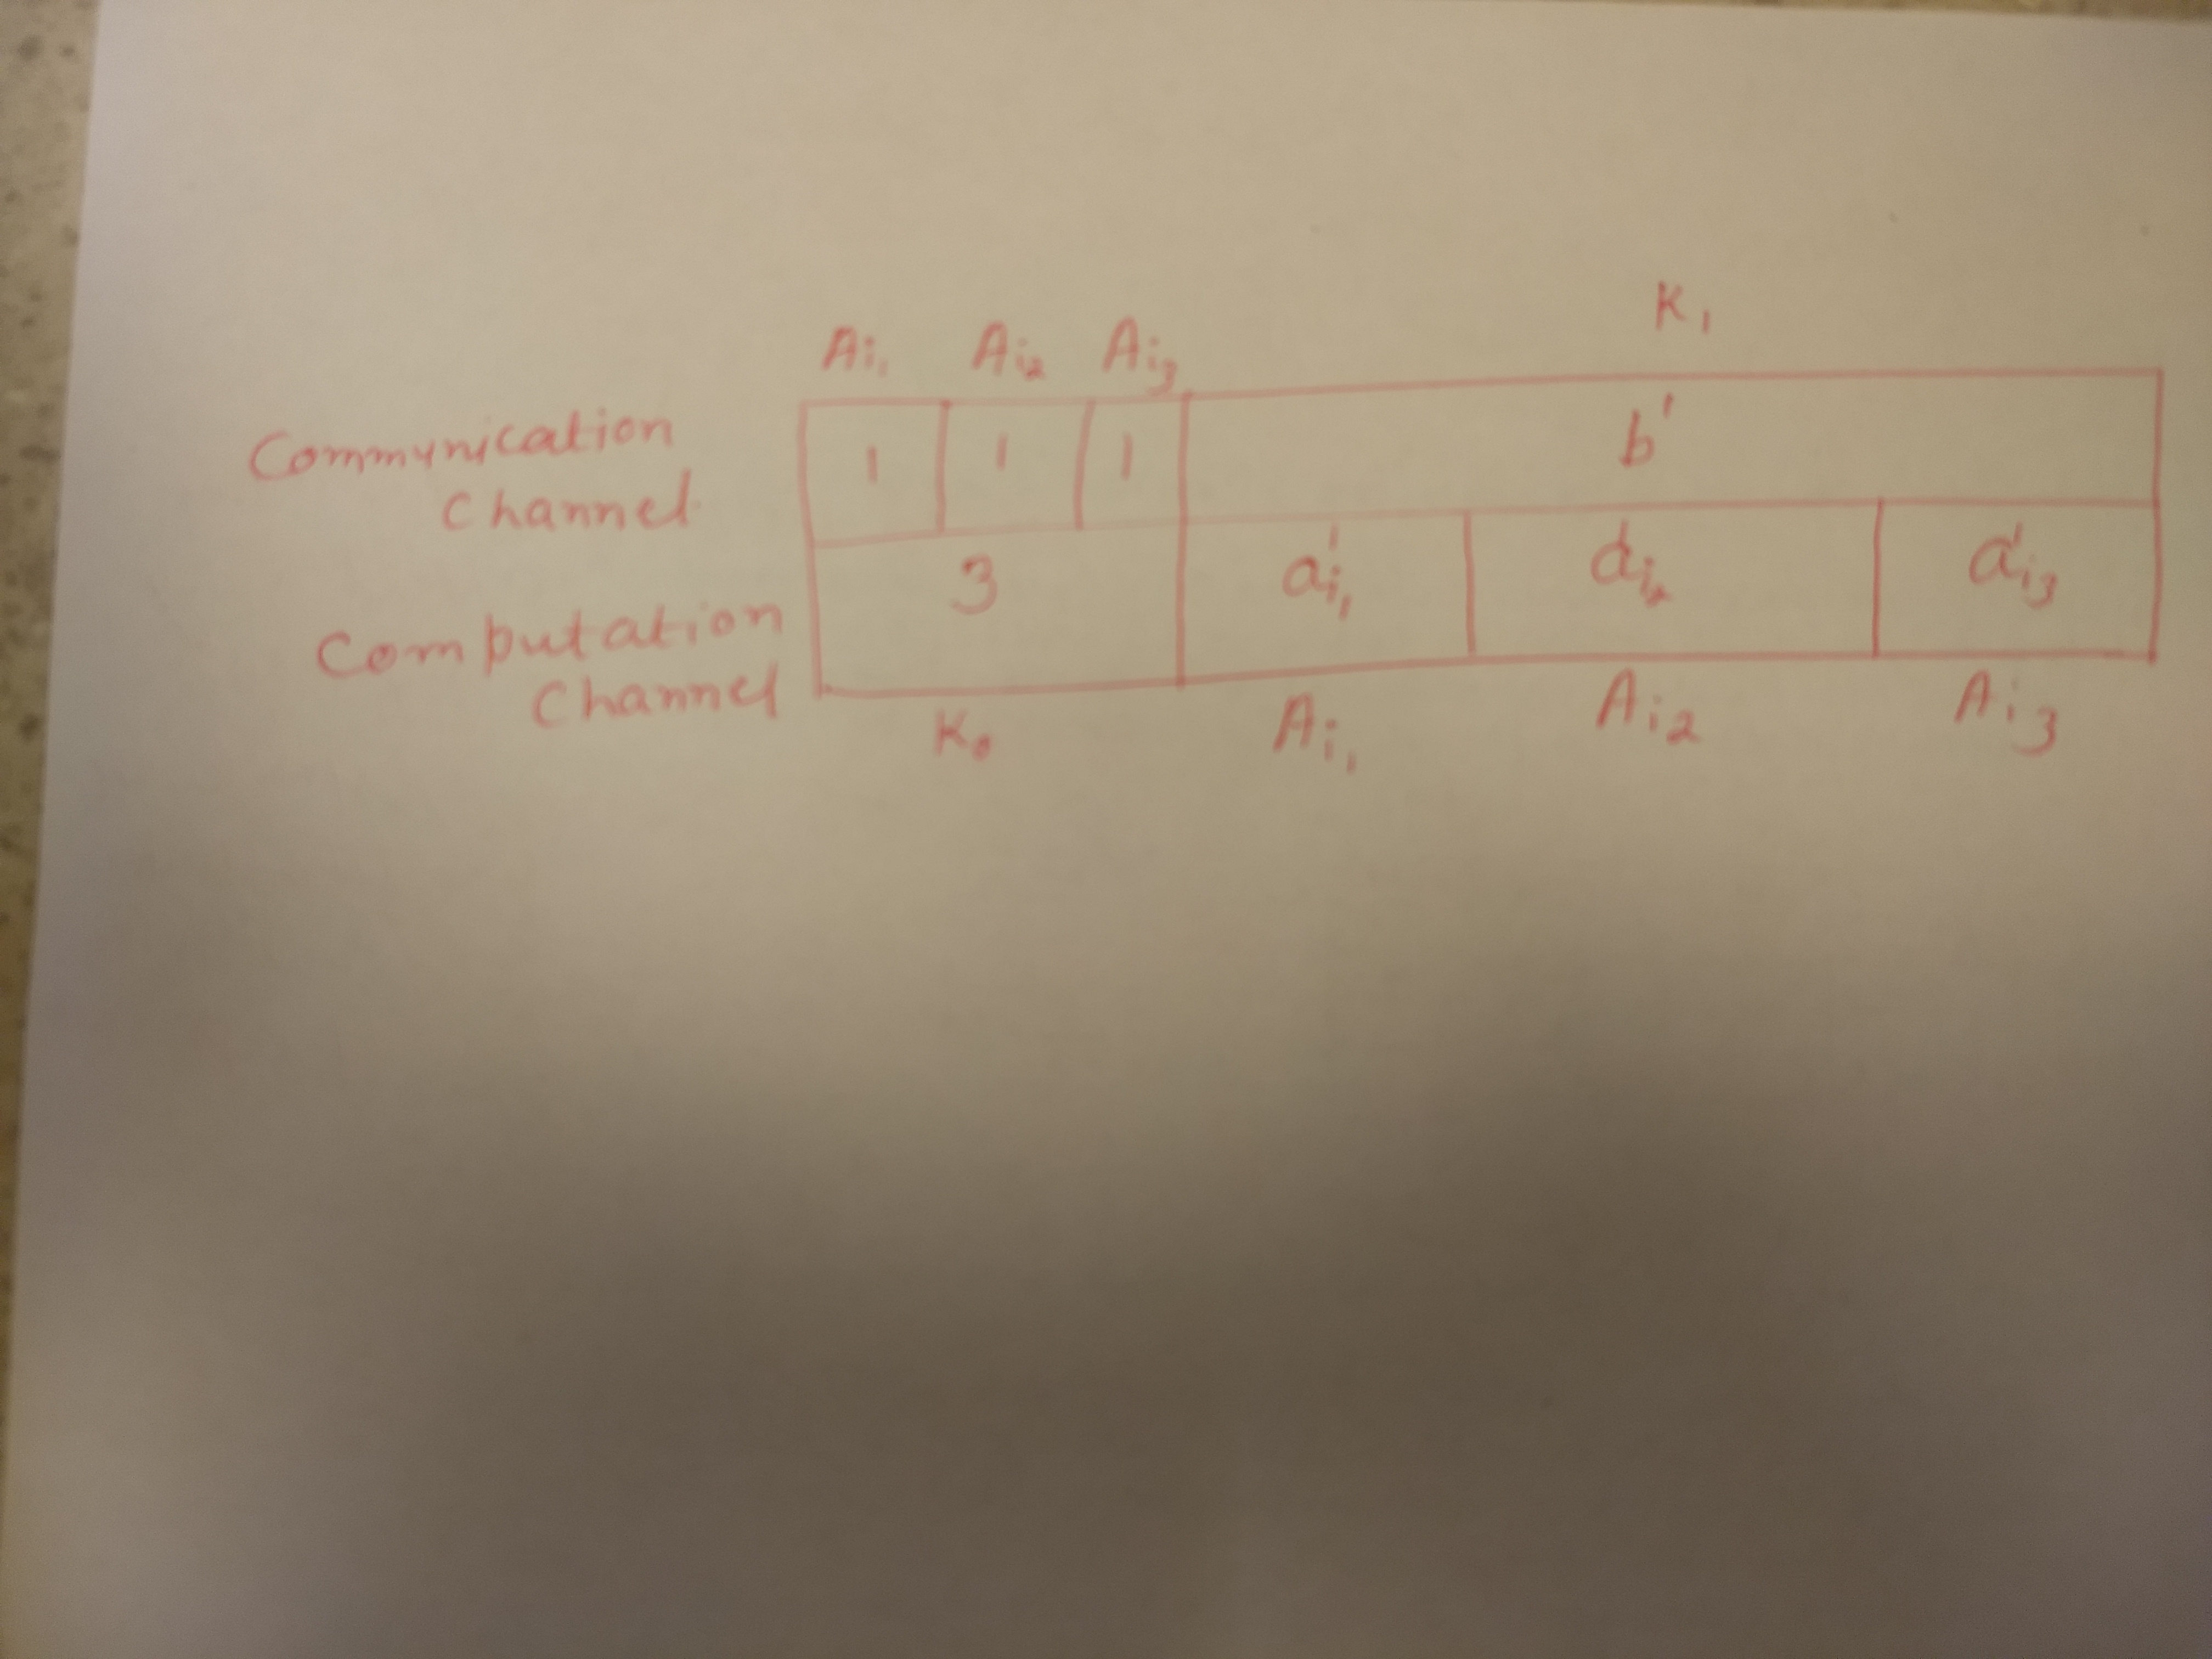
\includegraphics[scale=0.07]{Figs/3PARToSched.jpg}
   		\caption{ \label{fig:firstSegment} First segment of Schedule $S$}
   	\end{figure}
   	
   \end{proof}

Each task may require some intermediate buffer. As problem $DT$ is NP-complete and intermediate 
memory requirement of each task is zero (which is a special case of problem with intermediate memory 
requirement). Hence, problem $DT$ with intermediate memory requirement is also NP-complete.





The proof of the above theorem is inspired from work by [Papadimitriou et. al], which applies a similar 
technique for 2-machine flowshop problem, where each machine can hold fixed amount of jobs. The 
main difference with the our approach is that they consider unit buffer requirement on 1st machine 
after job completion. On the contrary, our approach is designed where there is not any restriction on 
requested input data and memory is acquired before starting the data transfer on communication 
channel(1st machine).





	
	
	\section{Order of Data Transfer and Computation heuristics}
	\begin{itemize}
		\item Talk about optimal strategy
		\item Order of computations and communications are same
		\item Static strategy
		\item Dynamic strategies
		\item Combination of Static and dynamic strategies
		\item strategies based on linear program 
	\end{itemize}

The heuristic proposed in the Section provides the optimal makespan when there is not any constraint on memory capacity. This optimal value indicates a lower bound on the makespan. We use $optimal_makespan_infinite_memory$ to represent this value. We assess the efficiency of other proposed heuristics in limited memory capacity in Section~\ref{sec:exp} with respect to this lower bound, $optimal_makespan_infinite_memory$.


We classify our heuristics into mainly three categories. In the first category, the order of all computations and communications is computed in advanced and the same order is followed on both channels. While in the second category, the best suited next task is chosen based on different criteria. In the last category, which is based on combination of strategies of the other two categories, we precompute the order and try to follow it as much as possible, but when the precomputed schedule induces idle time then we look for the best suited next task. In all of our strategies (except linear programming based strategy) order of communications and computations, are same.

\subsection{Static Ordering}
In this class of strategies, we compute the order of both computations and communications in advance based on criteria such as communication time, compute time, accelerated tasks. After computing the order, we follow the same order on computation and communication channels and make sure that at each point in the schedule memory capacity is respected.


In strategy (cite optimal strategy), compute intensive tasks (step 1) are sorted in increasing order of communication times. It allows tasks to utilize the computation channel maximally and make enough space on communication channel to accommodate more communication intensive tasks with maximum overlap. Communication intensive tasks are sorted in decreasing order of communication time, which allows tasks to utilize the gap created on communicated channel. Hence,  in this section, we obtain the orders by sorting tasks based on different combinations of communication and computation times.

%%%%name = "optimal_time_infinite_case";
%%%%string alg_name="order_of_optimal_strategy_infinite_memory";
%%%%string alg_name="increasing_order_of_communication_strategy";
%%%%string alg_name="decreasing_order_of_computation_strategy";
%%%%string alg_name="increasing_order_of_communication_plus_computation_strategy";
%%%%string alg_name="decreasing_order_of_communication_plus_computation_strategy";
%%%%string alg_name="optimal_order_infinite_memory_largest_communication_task_respects_memory_restriction";
%%%%string alg_name="optimal_order_infinite_memory_smallest_communication_task_respects_memory_restriction";
%%%%string alg_name="optimal_order_infinite_memory_maximum_accelerated_task_respects_memory_restriction";
\begin{itemize}[a)]
	\item $order_of_optimal_strategy_infinite_memory $: Order of communications and computations is obtained by the infinite memory heuristic. At each point in the schedule memory capacity is respected. Hence the makespan of this heuristic may be completely different from $optimal_makespan_infinite_memory$.
	
	\item $increasing_order_of_communication_strategy$: Order is obtained by sorting all tasks in non-decreasing order of communication time. 
	
	\item $decreasing_order_of_computation_strategy$: Order is obtained by sorting all tasks in non-increasing order of computation time. 
	\item $increasing_order_of_communication_plus_computation_strategy$: Order is obtained by sorting all tasks in non-decreasing order of sum of communication and computation times.
	\item $decreasing_order_of_communication_plus_computation_strategy$: Order is obtained by sorting all tasks in non-increasing order of sum of communication and computation times.
	
\end{itemize}
\todo[inline]{SKumar: equivalent tikz figure}

\begin{figure}[htb]
	
	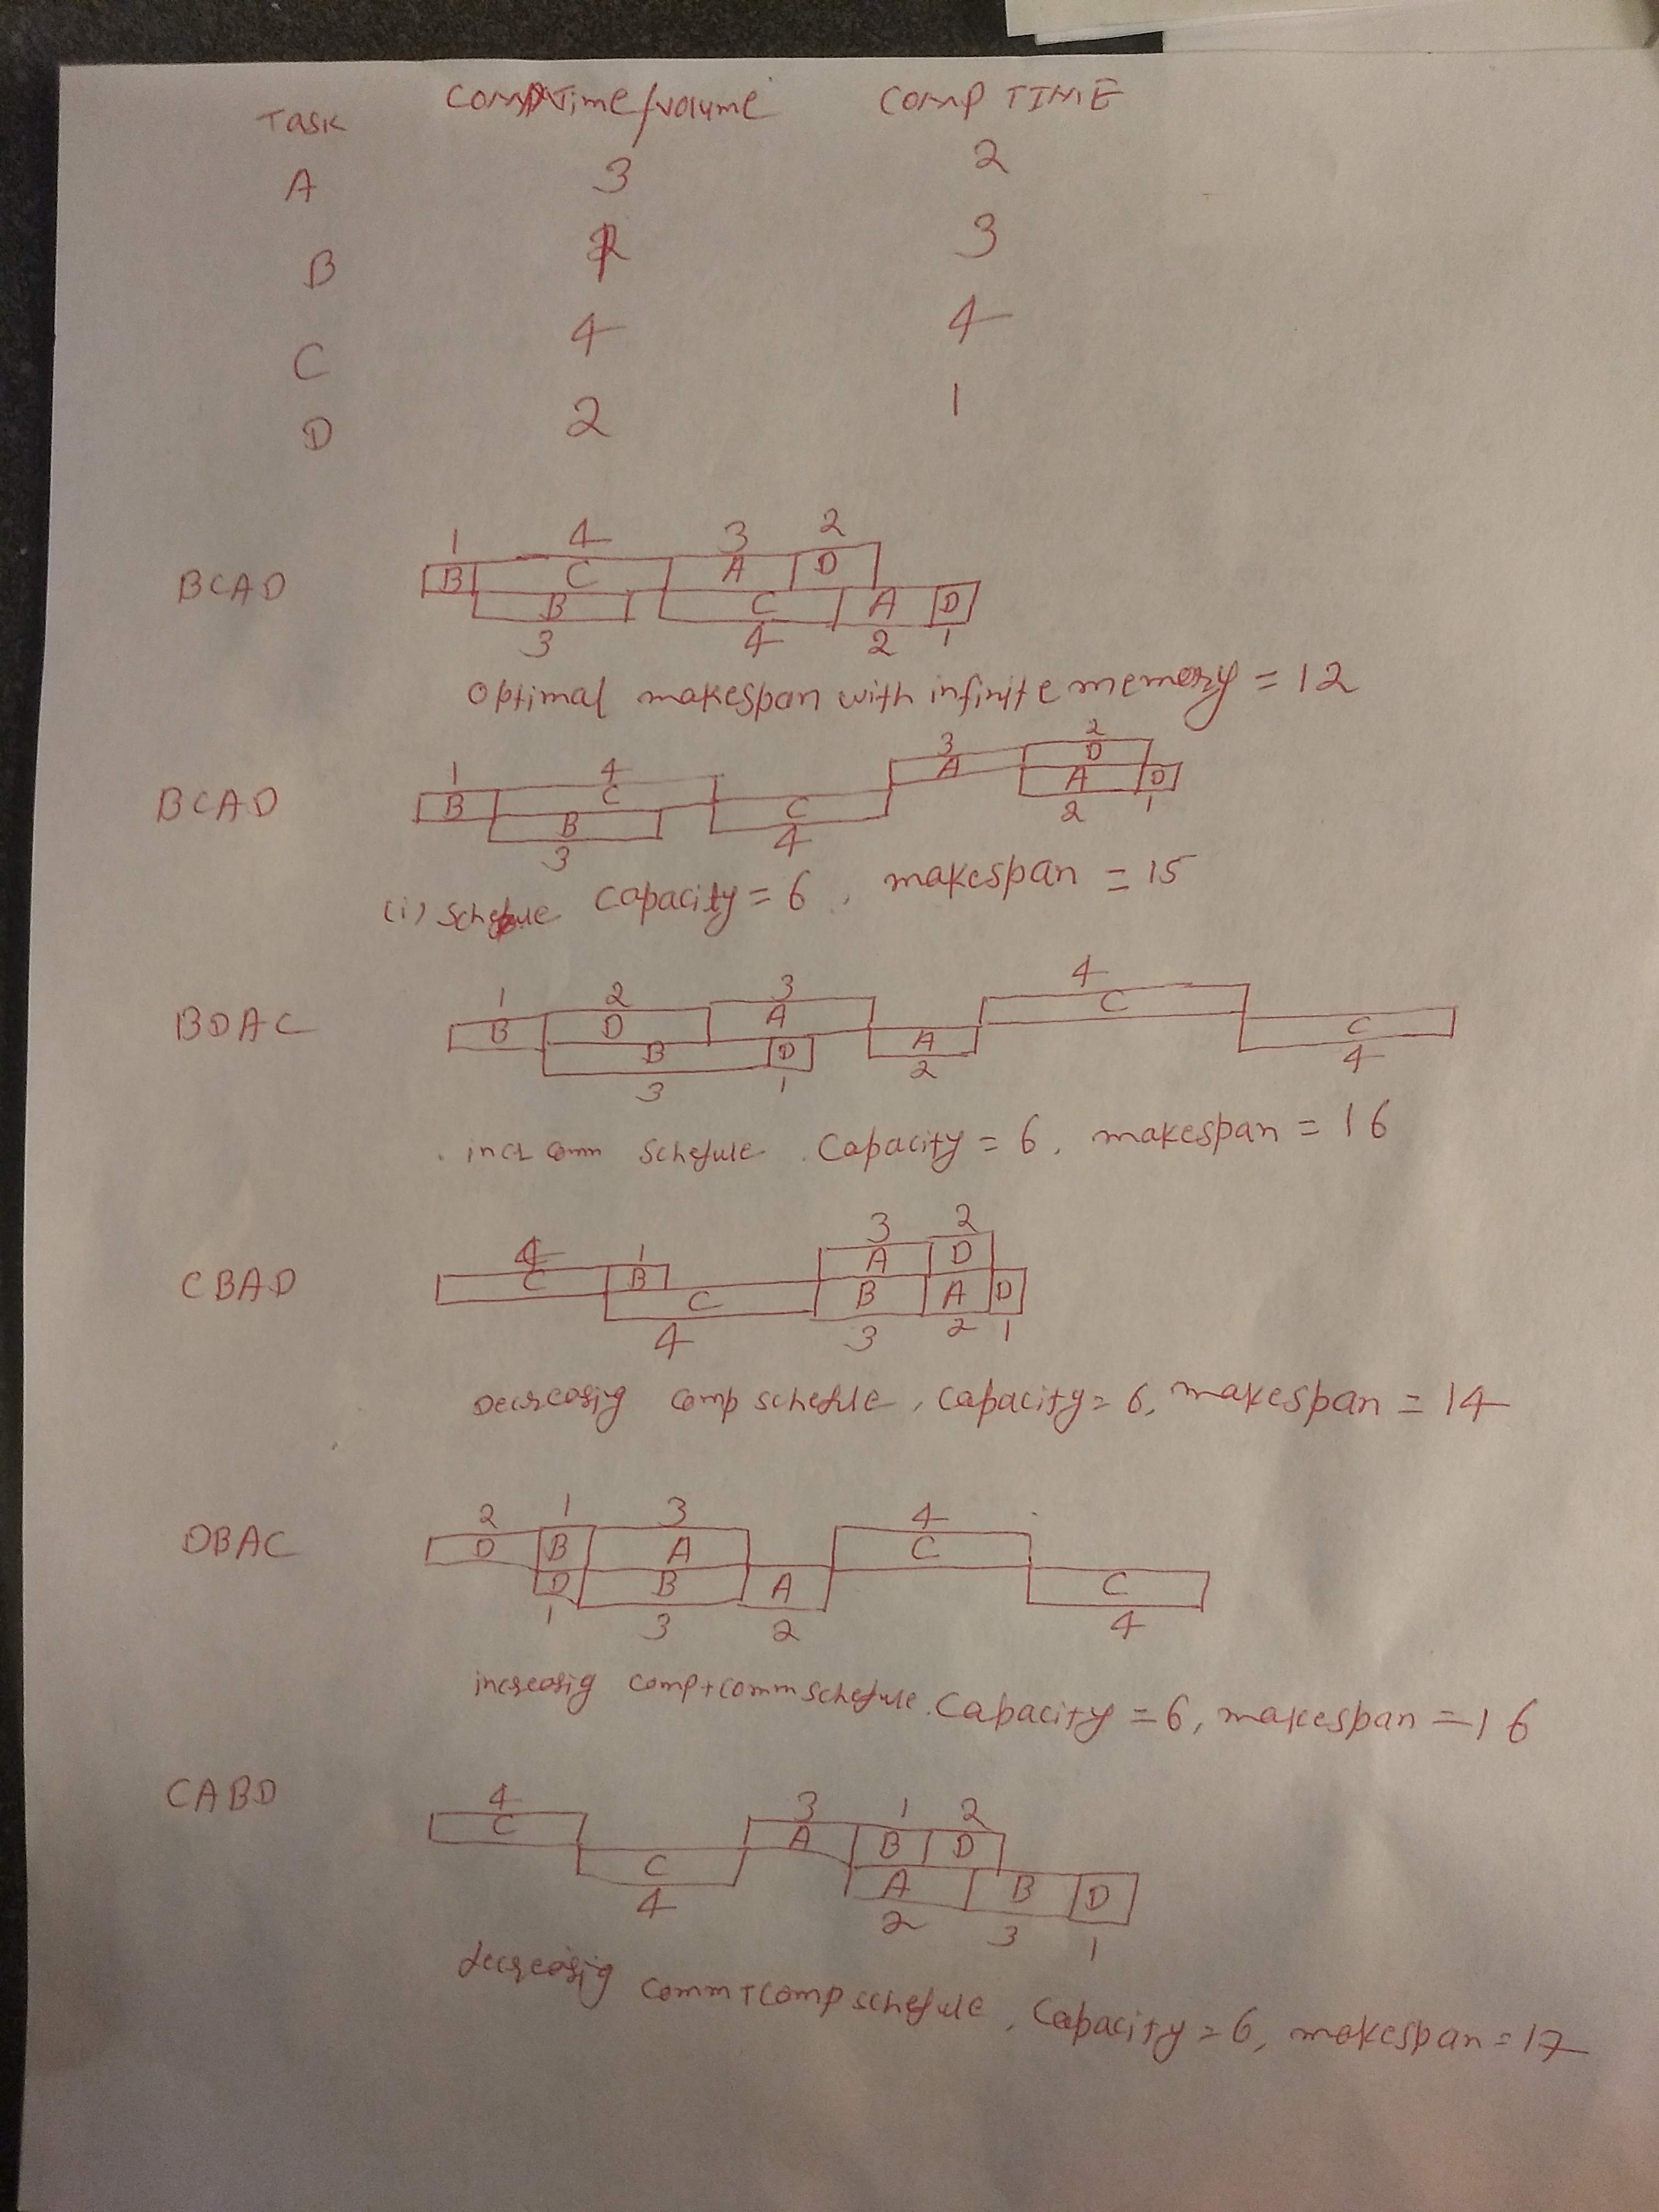
\includegraphics[scale=0.05]{Figs/staticOrderSchedules}
			\caption{Task set and schedules where orders are precomputed based on different heuristics.}
	\label{fig:staticOrderExample}
\end{figure}

Fig~\ref{fig:staticOrderExample} shows schedules for all proposed heuristics of this class for task set of Table (ref).
\subsection{Dynamic Selection}
%%%%string alg_name="largest_communication_task_respects_memory_restriction";
%%%%string alg_name="smallest_communication_task_respects_memory_restriction";
%%%%string alg_name="maximum_accelerated_task_respects_memory_restriction";

In this class of strategy, when communication channel is idle, a task is chosen which satisfies the selection criteria maximally among other tasks. For example, if the selection criteria is to choose a highly compute intensive task, than  we calculate the ratio of compute time and communication time for all tasks, and the task with the  maximum ratio is selected (ties are broken randomly). As we assume that order on both channels is same, hence order on compute channel will follow the order of communication channel.

\begin{itemize}[a)]
	\item $largest_communication_task_respects_memory_restriction$:  We select a set of tasks which induce minimum idle time on compute channel. A task with the largest communication time is chosen from this set.  Memory requirement of this task should not be more than presently available memory. 
	\item $smallest_communication_task_respects_memory_restriction$: A task with the smallest communication time is chosen.  Memory requirement of this task should not be more than presently available memory. 
	\item $maximum_accelerated_task_respects_memory_restriction$:  We select a set of tasks which induce minimum idle time on compute channel. A task with the maximum ratio of compute time to communication time  is chosen from this set.  Memory requirement of this task should not  be more than presently available memory.
	
\end{itemize}
\todo[inline]{SKumar: equivalent tikz figure}

\begin{figure}[htb]

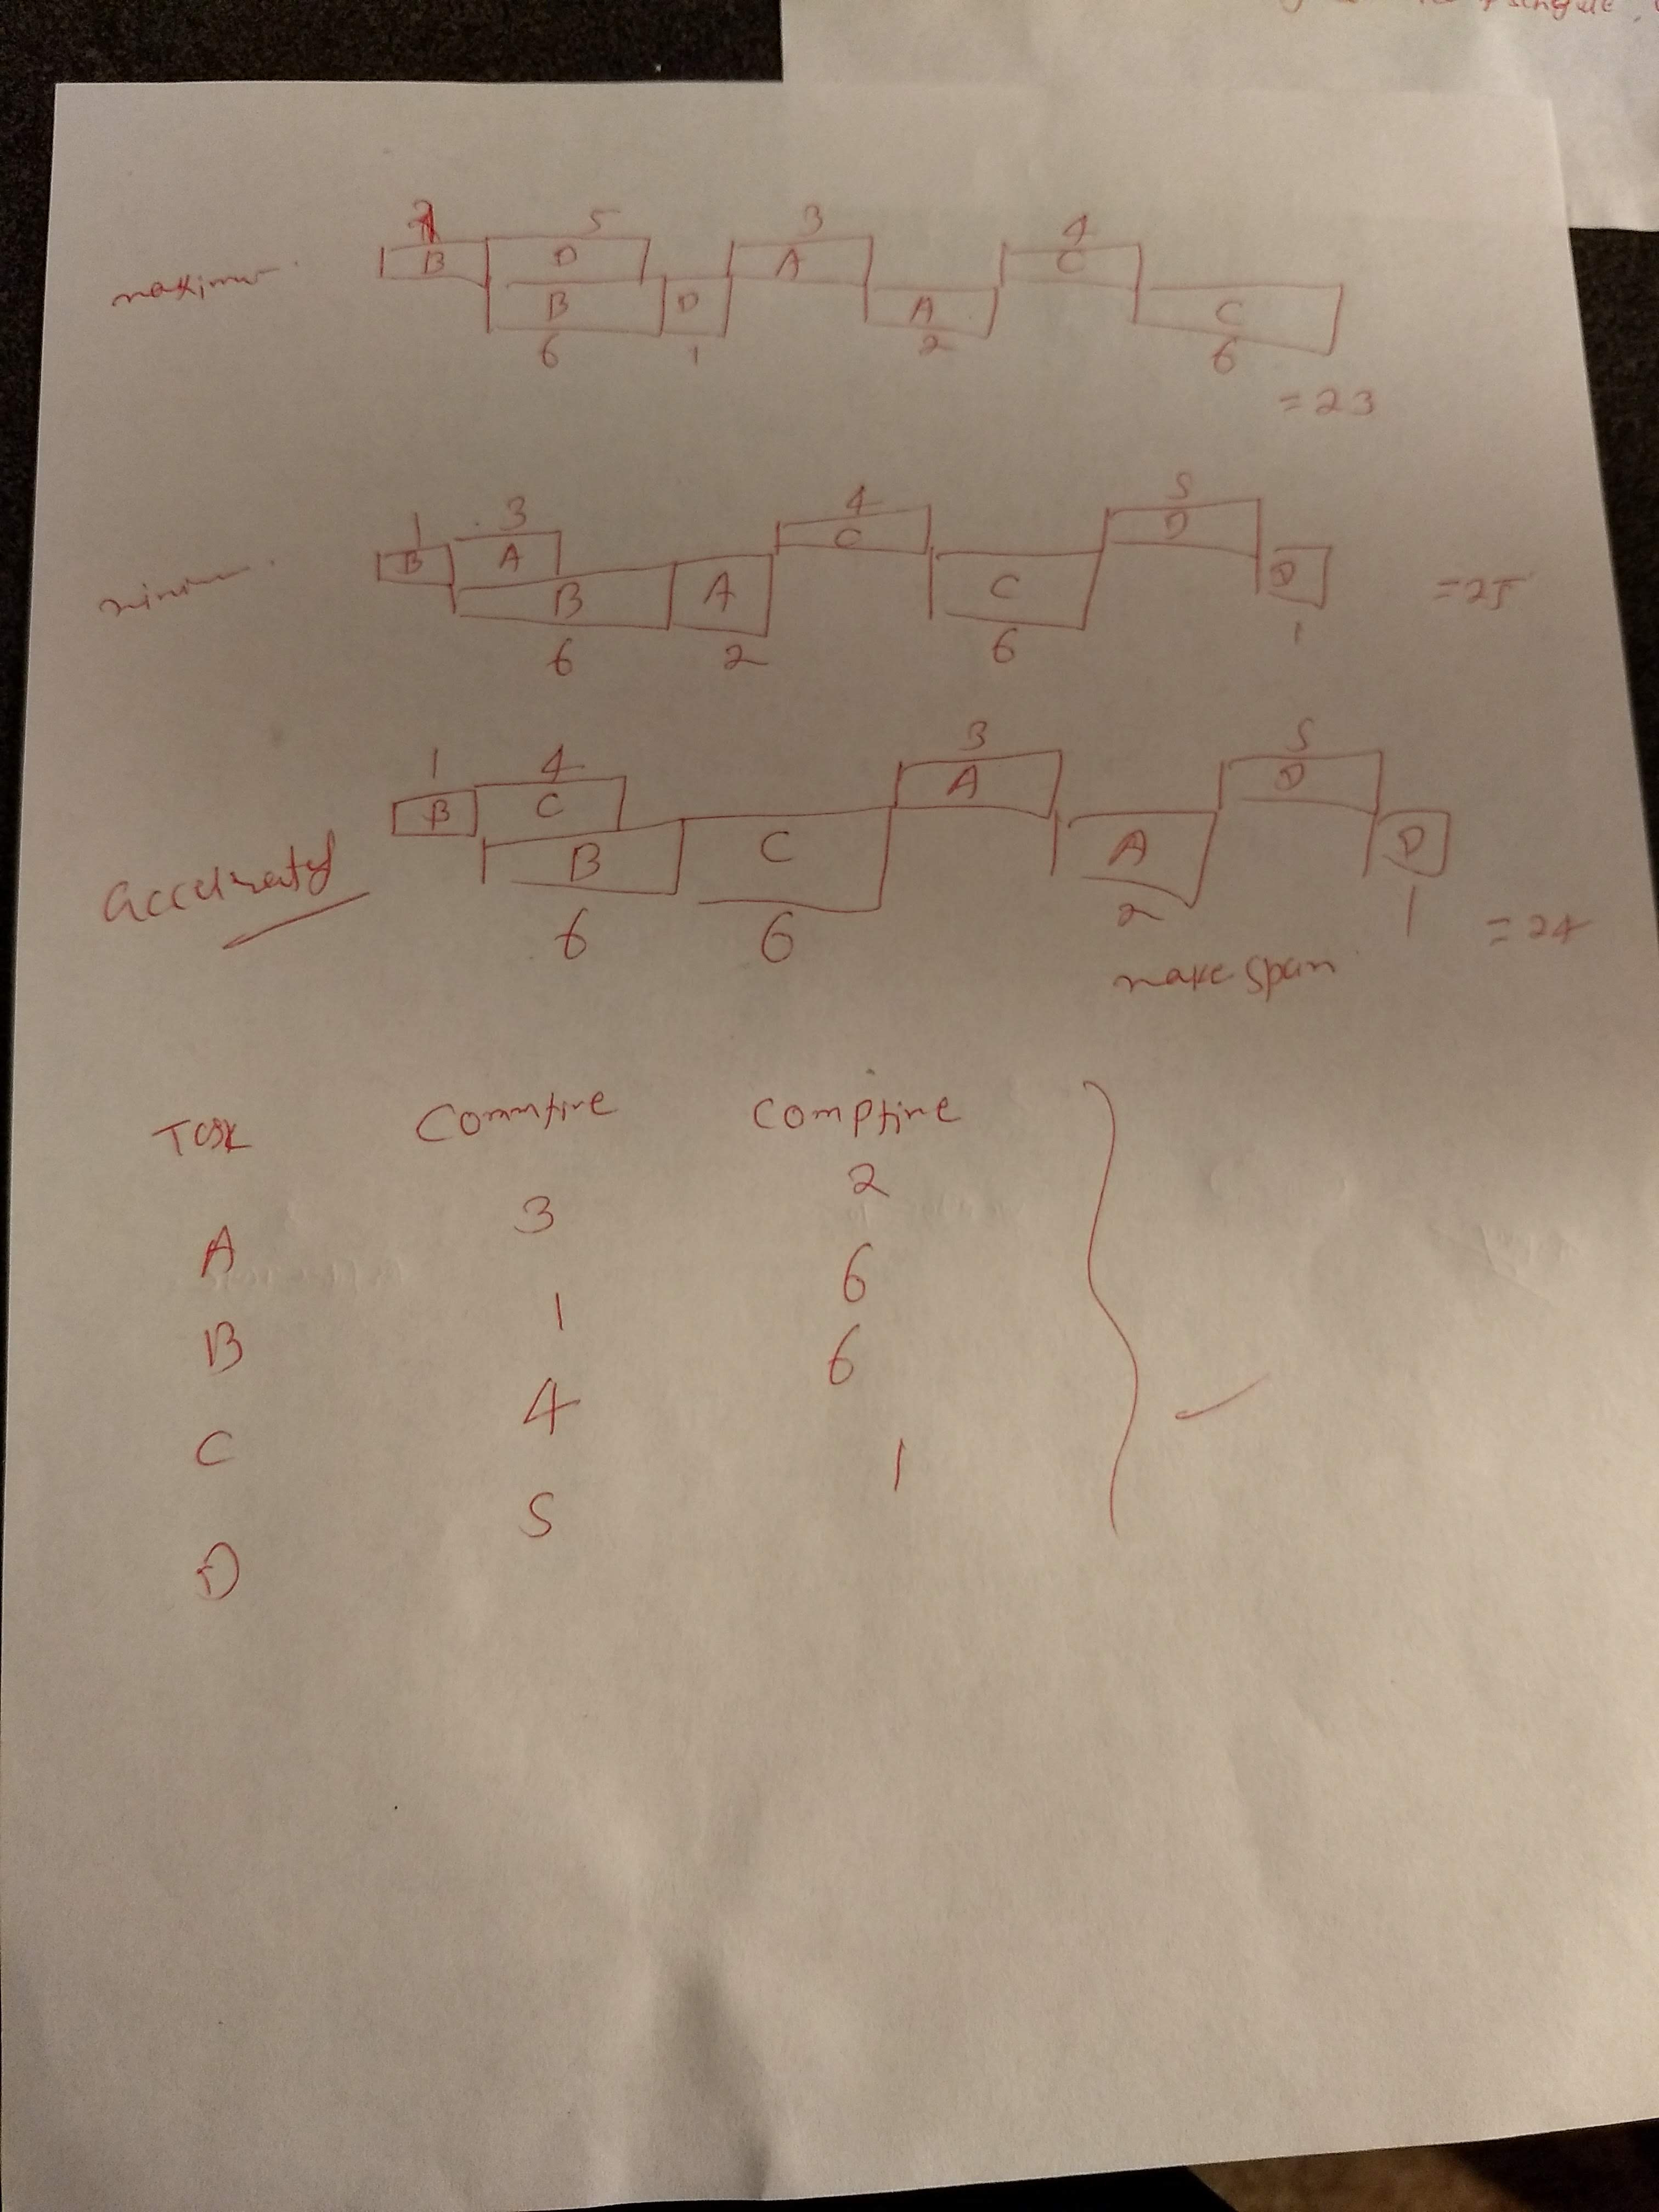
\includegraphics[scale=0.05]{Figs/dynamiSelectionSchedules}
\caption{Task set and schedules where orders are precomputed based on different heuristics.}
\label{fig:dynamicSelectionExample}
\end{figure}

Fig~\ref{fig:dynamicSelectionExample} shows schedules for all proposed heuristics of this class for task set of Table (ref).

\subsection{Static Order with dynamic Corrections}

In this class of strategy, we precompute the order of tasks based on different criteria and then try to follow the same order as much as possible. But when communication channel is idle due to memory requirement of the next task in the obtained order, then we select a task similar to previous strategy. After a task is selected then we update the remaining order without this task. This class of strategy takes advantage of  static information in the form of precomputed order and dynamic correction to minimize the idle time due to memory constraint.
%%%%alg_name="optimal_order_infinite_memory_largest_communication_task_respects_memory_restriction";
%%%%string alg_name="optimal_order_infinite_memory_smallest_communication_task_respects_memory_restriction";
%%%%string alg_name="optimal_order_infinite_memory_maximum_accelerated_task_respects_memory_restriction";

Initial order is obtained by infinity memory heuristic. When communication channel is idle due to memory requirement of the next task in the order, then we select a set of tasks which induce minimum idle time on compute channel and satisfy memory requirement. We define the following heuristics based on how we select a task from this set. After that order of remaining  tasks is updated without this task.

\begin{itemize}[a)]
	\item $optimal_order_infinite_memory_largest_communication_task_respects_memory_restriction$: A task with the largest communication time is chosen from the set.
	\item $optimal_order_infinite_memory_smallest_communication_task_respects_memory_restriction$:  A task with the smallest communication time is chosen from the set.
	\item $optimal_order_infinite_memory_maximum_accelerated_task_respects_memory_restriction$: A task,  whose ratio of compute time to communication time is maximum, is chosen from the set .
\end{itemize}


\todo[inline]{SKumar: equivalent tikz figure}
\begin{figure}[htb]
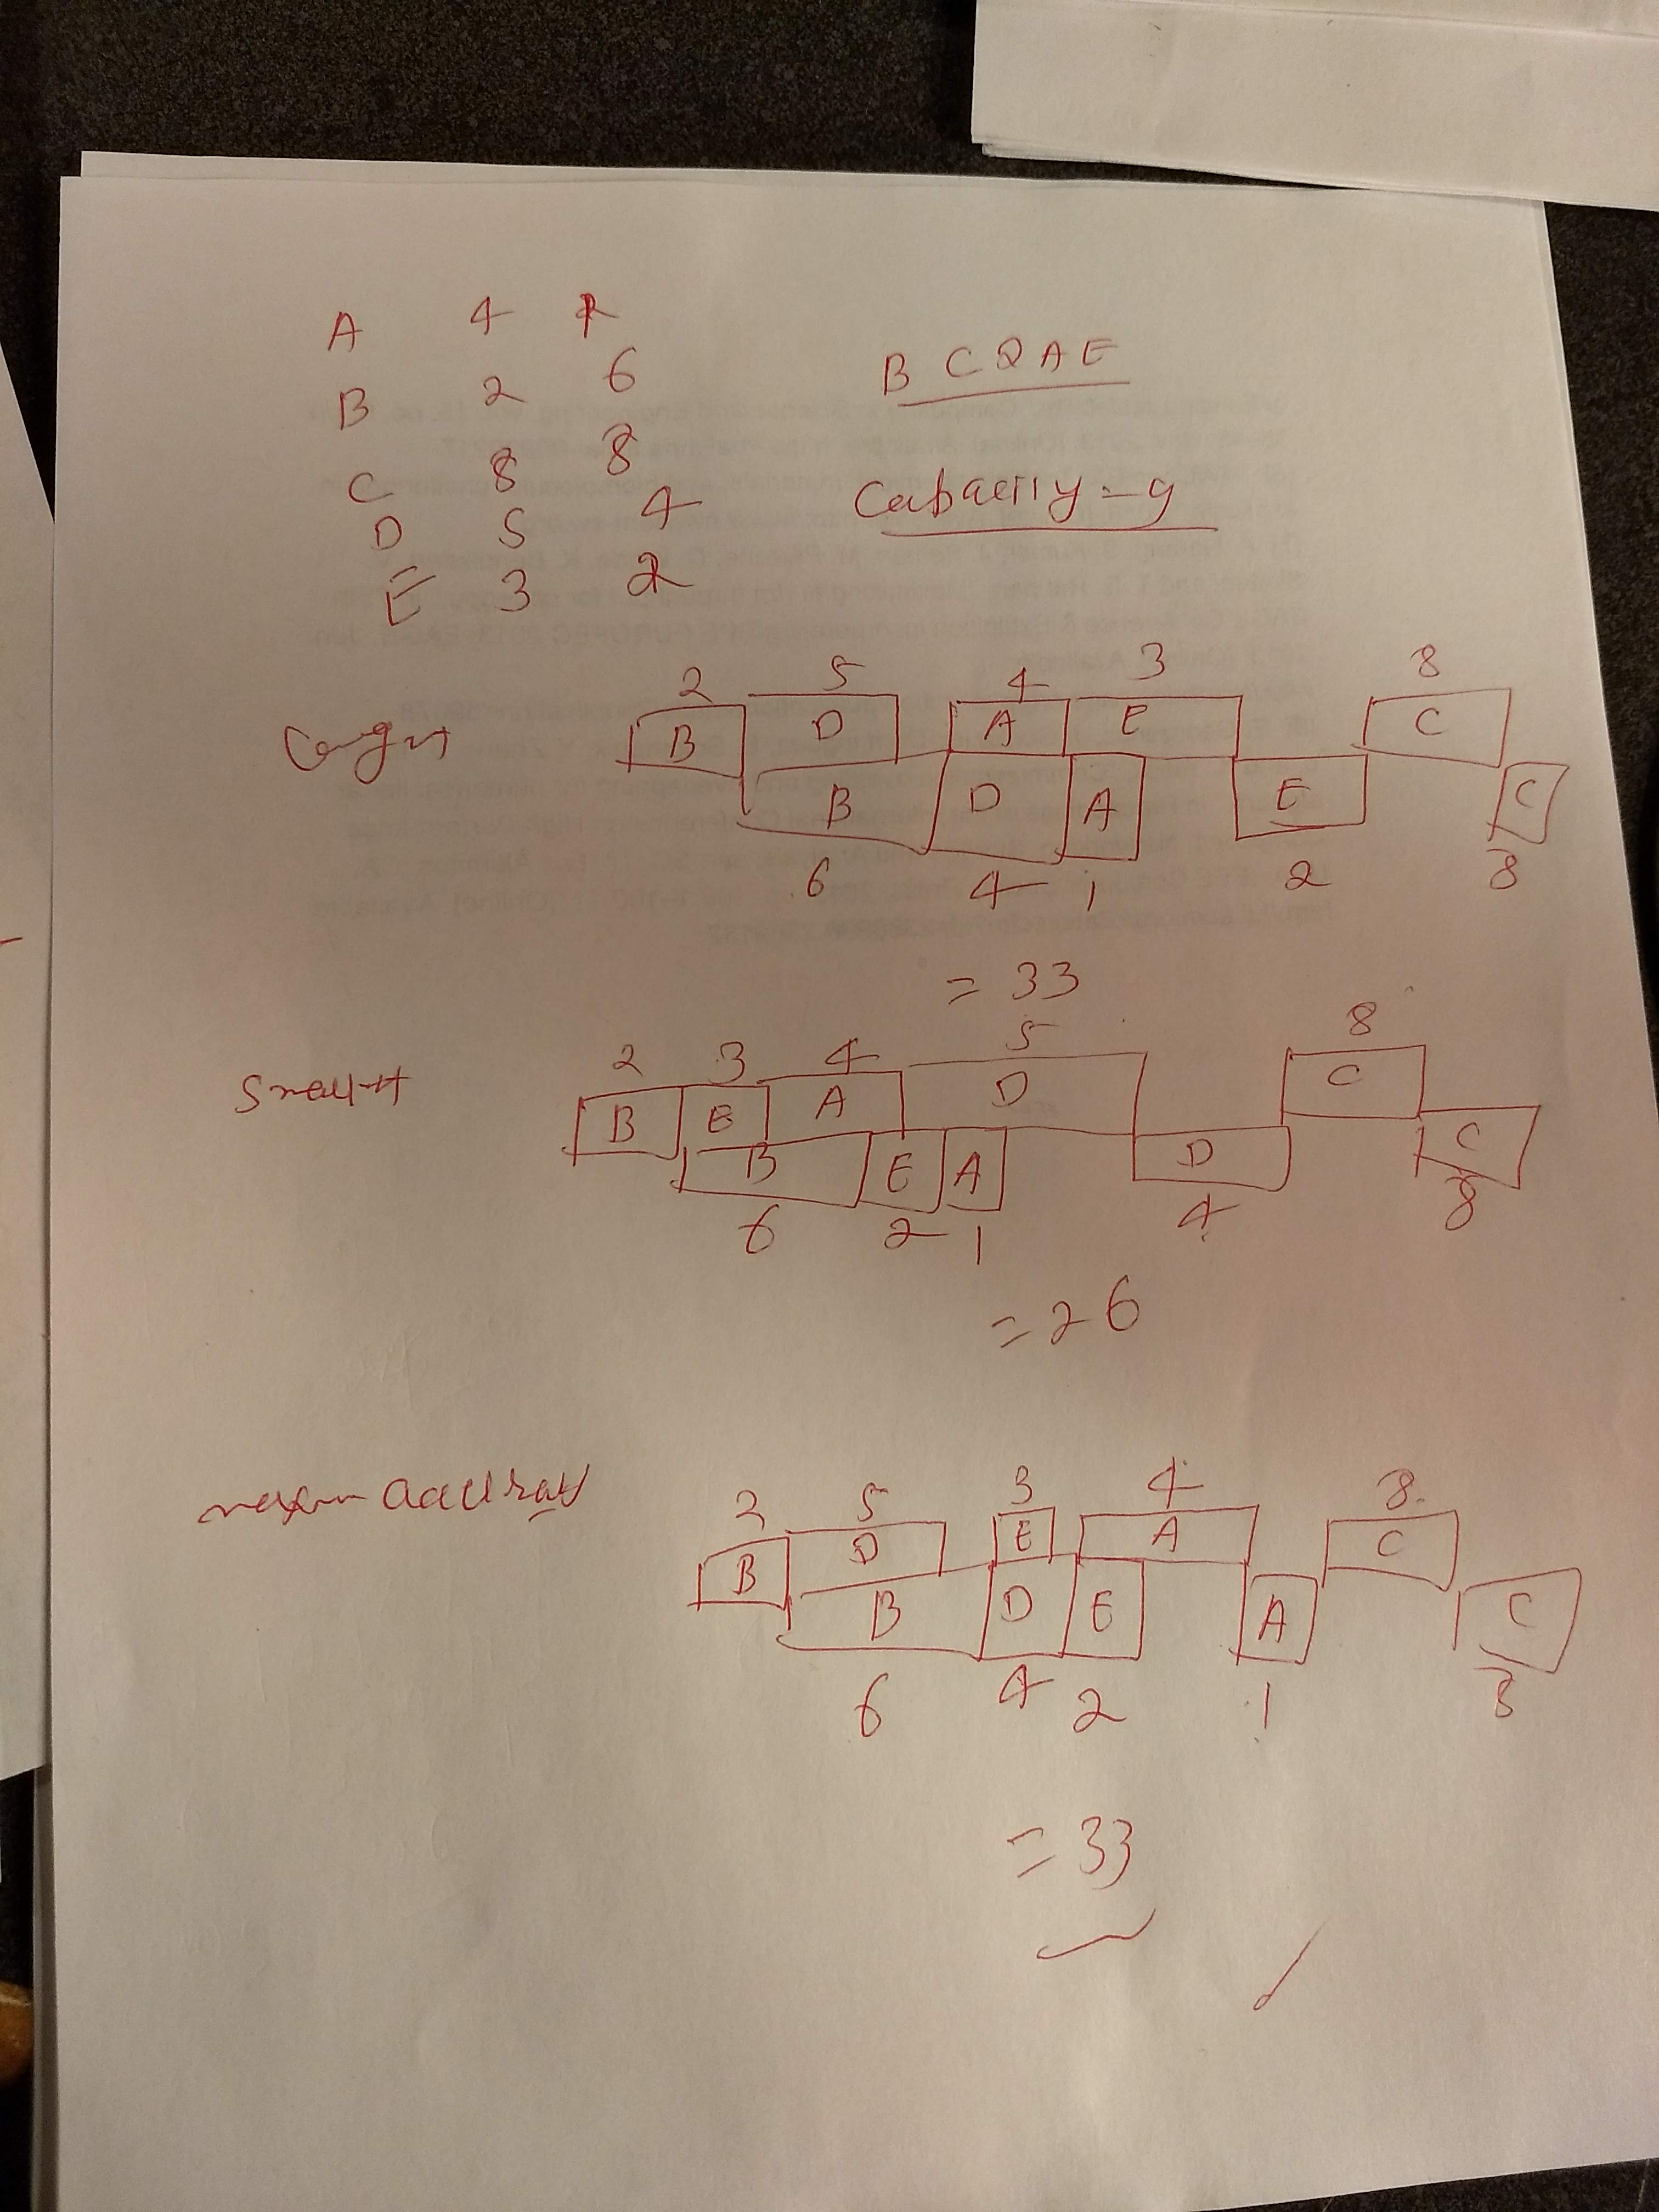
\includegraphics[scale=0.05]{Figs/staticOrderDynamicCorrectionsSchedules}
\caption{Task set and schedules where orders are precomputed based on different heuristics.}
\label{fig:staticOrderDynamicCorrectionsExample}
\end{figure}

Fig~\ref{fig:staticOrderDynamicCorrectionsExample} shows schedules for all proposed heuristics of this class for task set of Table (ref).




\subsection{Solving Linear Program Iteratively}
%%\subsection{Solving Linear Program Iteratively}
We use a mixed integer linear program  to obtain the order of data transfers and computations. We are unable to mange the optimal solution for the complete set $S$ in limited amount of time.  Hence, we construct and solve the linear program iteratively for a small subset of size $k$ . $CP(i)$ and $CM(i)$ represent computation and communication timings of task $T_i$. $TM(i)$ denotes intermediate memory requirement of task $T_i$ . Memory capacity of the  target system is $C$. In the linear program formulation, $s_i$ and $e_i$ (resp. $s'_i$ and $e'_i$) represent start and end time of communication (resp. computation) for task $T_i$. The formulation contains $i)$ n-1 boolean variables, $a_{ij}$, for each task $T_i$ to denote the order of $T_i$ and $T_j$  on communication channel   $ii)$ n-1 boolean variables, $b_{ij}$, for each task $T_i$ to denote the order of $T_i$ and $T_j$  on computation channel $iii)$ n-1 boolean variables, $c_{ij}$, for each task $T_i$ to denote the order of $s_i$ and $e'_j$, and $iv)$ (optional, if we consider temporary buffer requirement for each task) n-1 boolean variables, $d_{ij}$, for each task $T_i$ to denote the order of $e'_i$ and $s_j$.



\noindent Let $L=\sum_i (CP(i) + CM(i))$. It is evident that $e_i =s_i + CM(i)$ and $e'_i =s'_i + CP(i)$. The constraints are following.

\vspace*{-0.5cm}
\begin{align*}
& \text{minimize } l \text{ such that }\\
\forall i, \quad & \text{computation of task } T_i \text{ completes:}\\
& e'_i \leq l\\
\forall i, \quad & \text{computation stars after communication ends:}\\
& e_i \leq s'_i\\
\forall i, \forall j\ne i, \quad & \text{exclusive communication of task }T_i \text{ on communication channel:}\\
& e_j \leq s_i +(1-a_{ij})L\\
& e_i\leq s_j +a_{ij}L\\
\forall i, \forall j\ne i, \quad & \text{exclusive computation of task }T_i \text{ on computation channel:}\\
& e'_j \leq s'_i +(1-b_{ij})L\\
& e'_i\leq s'_j +b_{ij}L\\
\forall i, \forall j\ne i, \quad & \text{task }T_i \text{ respects memory capacity on communication channel:}\\
& e'_j \leq s_i +(1-c_{ij})L\\
& s_i< e'_j +c_{ij}L\\
& \sum_r (a_{ir} - c_{ir})CM(r) + CM(i) \le C\\
\forall i, \forall j\ne i, \quad & \text{task }T_i \text{ respects memory capacity on computation channel:}\\
& s_j < e'_i +(1-d_{ij})L\\
& e'_i\leq s_j +d_{ij}L\\
& \sum_r (d_{ir} - b_{ir})CM(r) + TM(i) \le C\\
\end{align*} 

\subsection{Favorable Situation for Heuristics}
\noindent The following table exhibits favorable scenarios for different heuristics. This table allows programmers to use the appropriate strategies to maximize communication-computation overlap for their applications.

\begin{table}[htb]
	\scriptsize
	\begin{tabular}{|c|p{3cm}|}
		\hline
		\textbf{Heuristic} & \textbf{Favorable Situation} \\ \hline
		order\_of\_optimal\_strategy\_infinite\_memory & Unlimited memory capacity (\textcolor{green}{Optimal}) \\ \hline
		increasing\_order\_of\_communication\_strategy & Unlimited memory capacity and tasks are compute intensive (\textcolor{green}{Optimal}) \\ \hline
		decreasing\_order\_of\_computation\_strategy & Unlimited memory capacity and tasks are communication intensive (\textcolor{green}{Optimal}) \\ \hline
		increasing\_order\_of\_communication\_plus\_computation\_strategy & Moderate memory capacity and most tasks are compute intensive \\ \hline
		decreasing\_order\_of\_communication\_plus\_computation\_strategy & Moderate memory capacity and most tasks are communication intensive \\ \hline
		largest\_communication\_task\_respects\_memory\_restriction &  Limited memory capacity and significant percentage of tasks are communication intensive \\ \hline
		smallest\_communication\_task\_respects\_memory\_restriction & Limited memory capacity and most tasks are compute intensive \\ \hline
		maximum\_accelerated\_task\_respects\_memory\_restriction &  Limited memory capacity and number of communication and compute intensive tasks are approximately equal \\ \hline
		optimal\_order\_infinite\_memory\_largest\_communication\_task\_respects\_memory\_restriction & Moderate memory capacity and significant percentage of tasks are communication intensive\\ \hline
		optimal\_order\_infinite\_memory\_smallest\_communication\_task\_respects\_memory\_restriction & Moderate memory capacity and most tasks are compute intensive \\ \hline
		optimal\_order\_infinite\_memory\_maximum\_accelerated\_task\_respects\_memory\_restriction & Moderate   memory capacity and number of communication and compute intensive tasks are approximately equal \\ \hline
	\end{tabular}\caption{~\label{tab:heuristicsAndFavorableScenarios}Heuristics and their favorable scenarios}
\end{table}


Here moderate memory capacity refers to limited capacity but close to the maximum memory  requirement of the considered application.





	\section{Experimental Results}
	\label{sec:exp}
	
	\todo[inline]{Machine information and our model}
	
	We consider a machine called Cascade, available at PNNL, for our experiments. We obtain traces by running  two molecular chemistry applications,  double precision version of Hartree-Fock (HF) and Coupled Cluster Single Double (CCSD) of NWChem package with 4 Uracil molecules input on 10 nodes of this machine. Each node is composed of 16 Intel Xeon E5-2670 cores, hence we use 160 processes for the execution. Each process executes 300-800 tasks.  NWChem takes advantages of a Partitioned Global Address Space Programming Model, Global Arrays (GA), to use shared-memory programming APIs  on distributed memory computers.  Our data transfer model is quite simple and  we consider that all data transfers between each process's local memory and GA memory take the same route. Modeling of different routes of data transfers for the same source-destination pair, bandwidth sharing for different source-destination pairs and network congestion is more challenging and part of our future work. Our model is simple yet it provides insight to the application developers (or runtime system) that  in what-order all data transfer  are issued for the same source-destination pair to maximise communication-computation overlap. Our model is easily adaptable to any source-destination where there is one fixed route between source and destination (such as between CPU and GPU, one copy engine to transfer data from CPU (resp. GPU) to GPU (resp. CPU) ).
	\todo[inline]{More about tiling}
	Both applications mainly perform two types of computations, tensor transpose and tensor contractions.  HF expects to specify a tile size and we set it to 100, so that each core can be efficiently utilize.  CCSD automatically determines tile sizes at different program points based on the input (molecule?).  Hence, HF operates on almost homogeneous tiles while CCSD on heterogeneous tiles.
	
%%	\todo[inline]{Scheduled based on Gilmore-Gomory algorithm and its performance }
	We also consider an algorithm, proposed by Gilmore and Gomory, to obtain the minimal cost sequence for a set of jobs. In this algorithm, each job has a start and end state and a cost is associated to change the state. In our context, this cost can be seen as non-overlap time of computation for two adjacent jobs. Here is the main idea of this algorithm. Initially partial sequence of jobs is represented by a graph such that their overlap is maximum. Subsequently edges are added to this graph which minimized the total non-overlap cost  and connects two components. When all nodes of this graph is connected then an edge interchange mechanism is taken into account to determine the sequence of jobs, which ensures that the sequence has minimal cost.
	
	We refer ~\cite{Gilmore-Gomory:1964} for the detailed algorithm and ~\cite{gitworkrepo} for our implementation. This algorithm does not take memory capacity into consideration and only provides the sequence of processing. We applied the same sequence with different memory capacity restrictions for our experiments and call this heuristic as \textit{Gilmore-Gomory}.
	
	\todo[inline]{may convert 10 subplots to 8 in all performance diagrams}
	\todo[inline]{increase font size in all plots, may be free scale-y}
	\todo[inline]{SKumar: decide metrics: ratio to optimal, percentage overlap, 100 - percentage non overlap}
	
	
	IWe evaluate different data transfer heuristics for the several memory capacities. From the obtained traces, first we determine the minimum requirement of the memory capacity $m_c$ to execute all tasks. Then we observe the behavior of all heuristics with memory capacity  $m_c$ to $2m_c$, in the gap of $0.1m_c$. Our performance metric is $ratio\_to\_optimal$, which is defined as the following. Let the makespan of a heuristic $H$ is $M_H$ and the makespan of the $optimal  case$ with infinite memory is $M_O$, then  $ratio\_to\_optimal (H)$ is $\frac{M_H}{M_O}$ (lower value is better). This value would be  greater or equal to $1$. A value closer to $1$ indicates that suitability of a particular heuristic and maximum possible communication-computation overlap has been achieved for that heuristic.
	
	
	Figures ~\ref{fig:ratio_to_optimal_hf} and ~\ref{fig:ratio_to_optimal_ccsd} depict the distribution of the performance  of each heuristic for all considered memory capacities, where plots are categorized by memory capacities. For each memory capacity and each heuristic, the box on the plot displays the median, first and last quartile, and the whiskers indicate minimum and maximum values, with outliers are shown by black dots.
\subsection{HF Performance}	
	\begin{figure}[htb]
		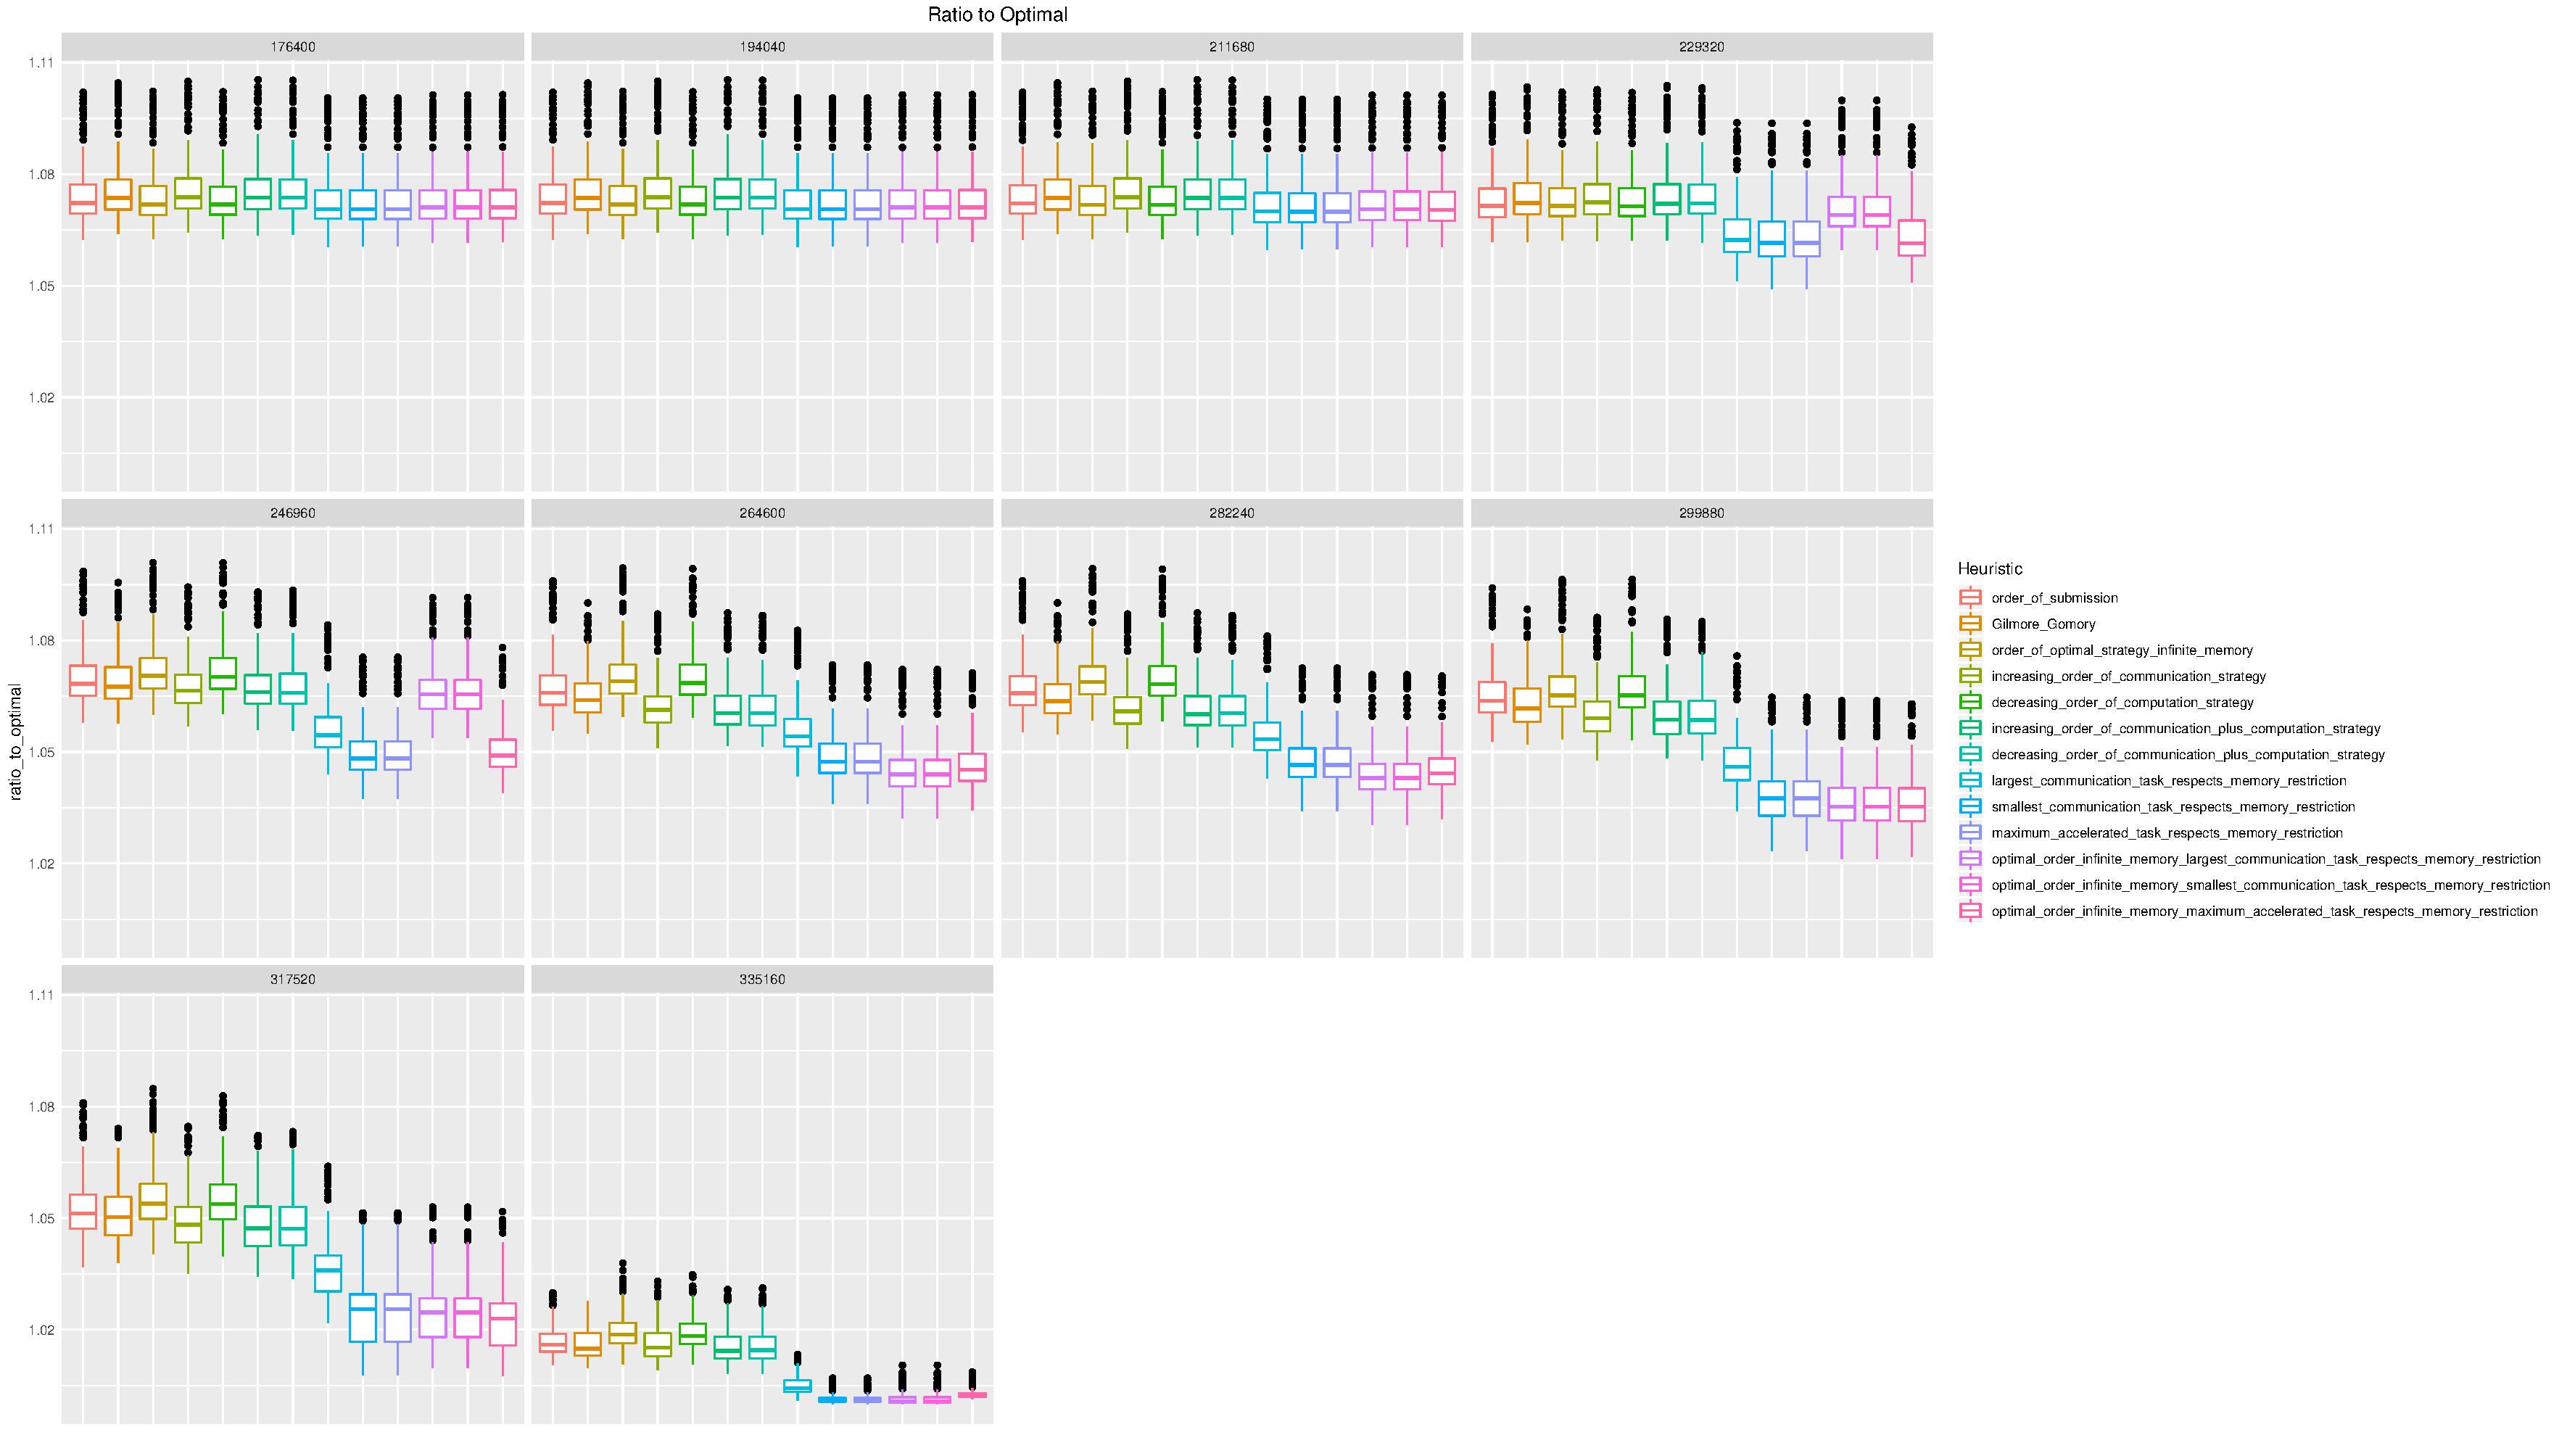
\includegraphics[scale=0.3]{../ExperimentalResults/ratio_to_optimal_hf.pdf}
		\caption{Comparison of different heuristics for HF.}
		\label{fig:ratio_to_optimal_hf}
	\end{figure}
 As indicated above, HF tasks are highly homogeneous, this is also noticeable in Figure~\ref{fig:ratio_to_optimal_hf}. All heuristics depict similar behavior for minimum memory capacity $m_c$  and  increasing the memory capacity slightly does not change the performance of all heuristics. As memory capacity increased further, dynamic variants of heuristics starts performing better and for the moderate memory capacities (close to $2m_c$ ), staticOrderDynamicCorrection variants outperforms others. \textit{Gilmore-Gomory} heuristic does not achieve good performance. it can be understand from the fact that task sequence is obtained considering no extra memory is available, but here we apply the same sequence for a different scenario,  overall memory consumed at each point is limited to memory capacity.


	\begin{figure}[htb]
	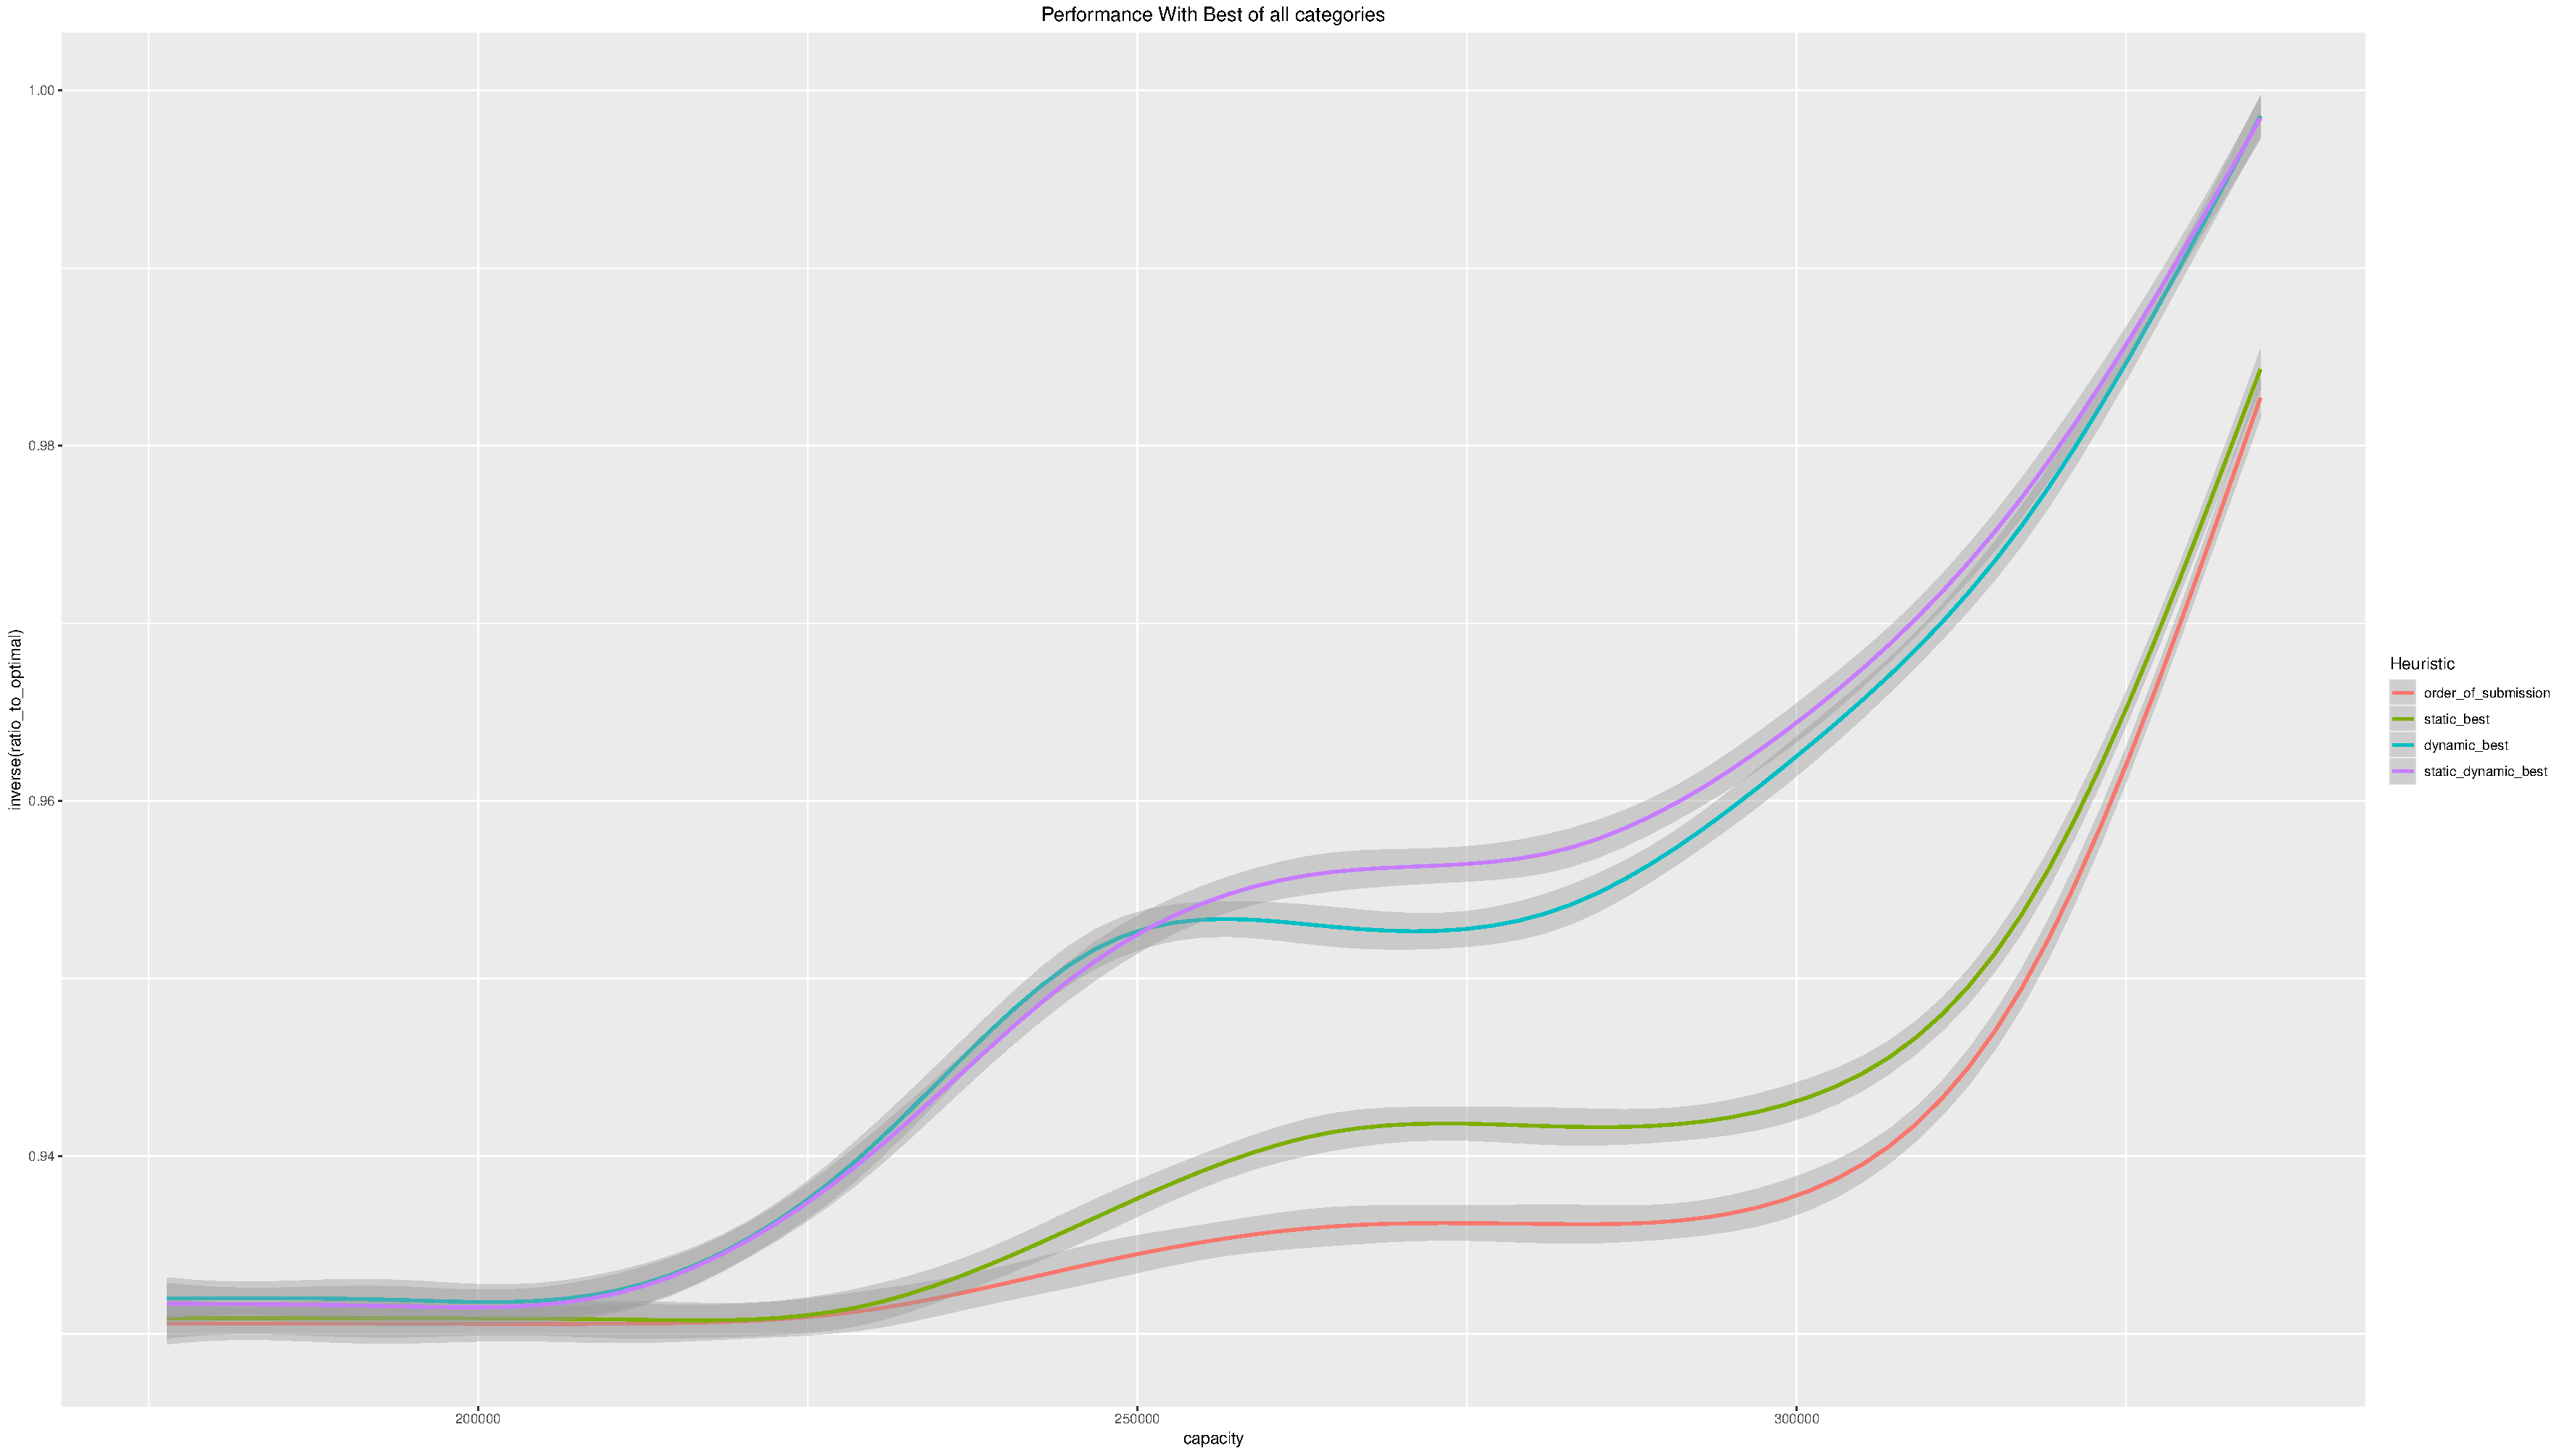
\includegraphics[scale=0.25]{../ExperimentalResults/inverse_ratio_to_optimal_hf-best.pdf}
	\caption{Comparision of best variants of all categories for HF.}
	\label{fig:ratio_to_optimal_best_hf}
	\end{figure}

 
Figure~\ref{fig:ratio_to_optimal_best_hf} shows the performance comparison of best variants of all categories with the $order_of_submission$ strategy. Static strategies are expected to perform better when there is not any memory capacity restriction, hence this plot indicates that static strategies face capacity bottleneck and underperform. Dynamic strategies achieve better performance with limited memory capacity and staticOrderDynamicCorrection  strategies suit in moderate memory capacity scenarios.

\subsection{CCSD Performance}

	\begin{figure}[htb]
	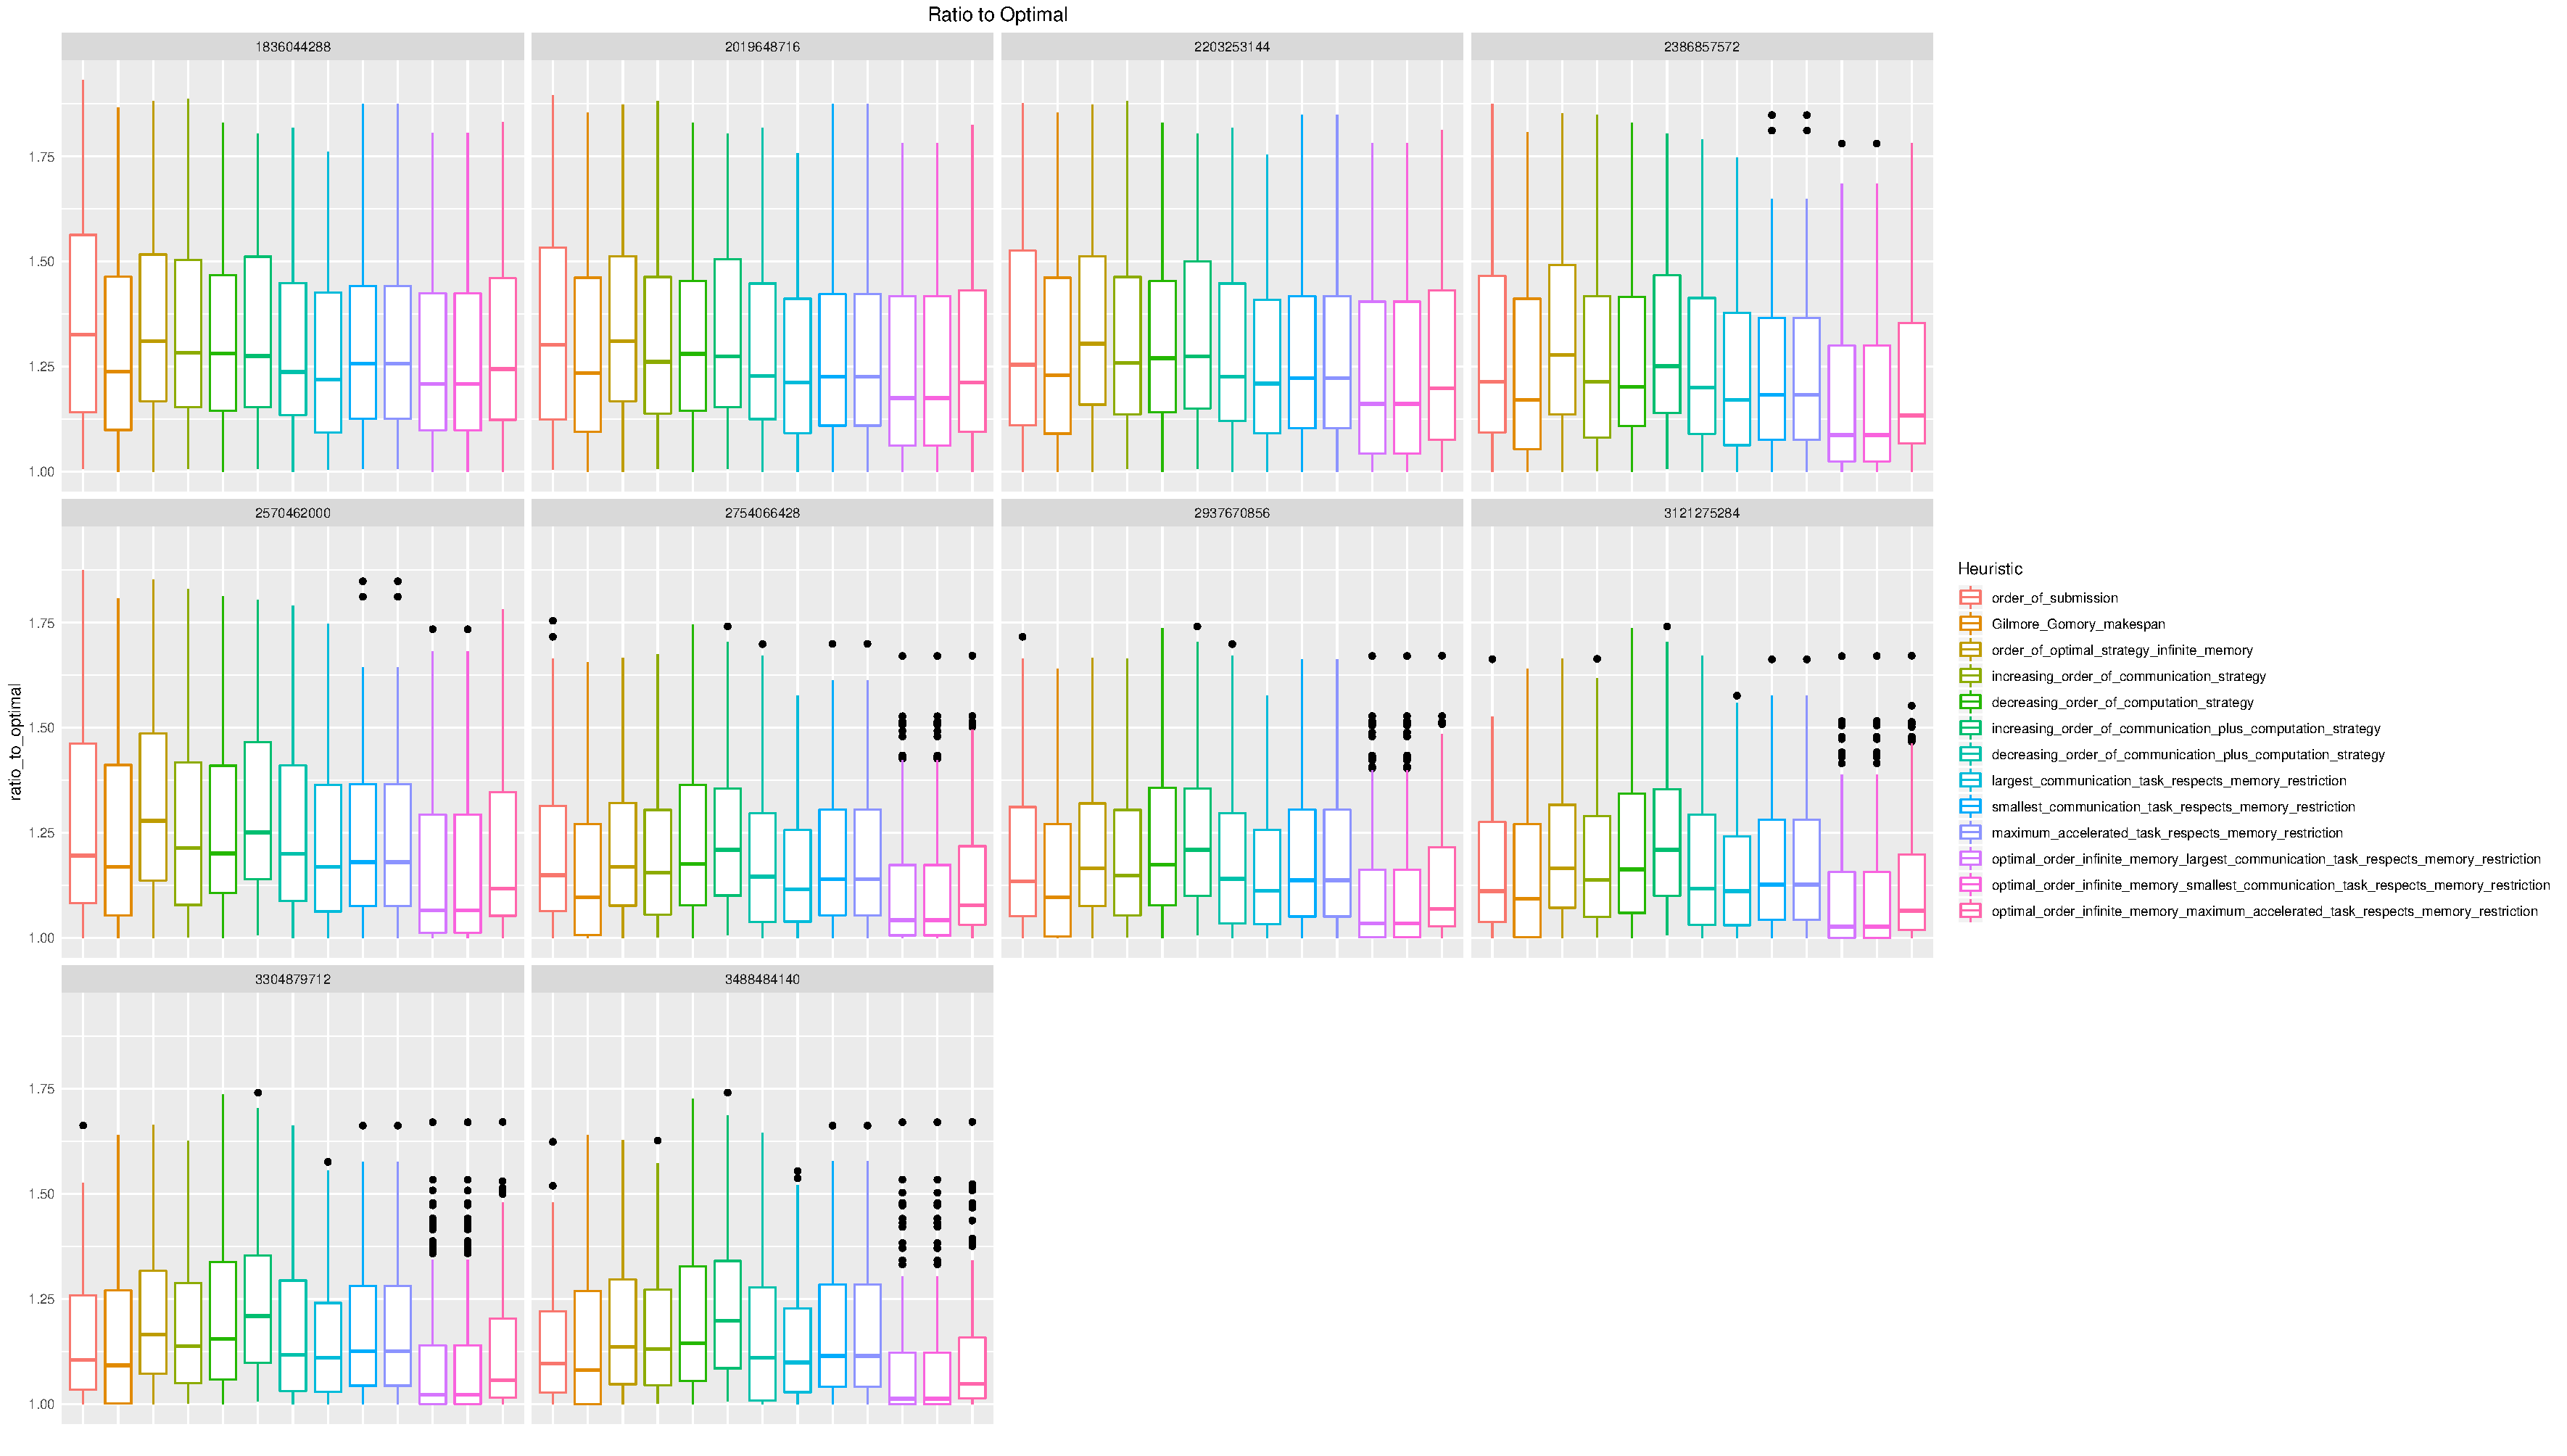
\includegraphics[scale=0.3]{../ExperimentalResults/ratio_to_optimal_ccsd.pdf}
	\caption{Comparison of different heuristics for CCSD.}
	\label{fig:ratio_to_optimal_ccsd}
	\end{figure}	

CCSD application operates on tasks of different sizes, hence different heuristics depict distinct behaviors even at minimum memory capacity $m_c$ . Heterogeneity favors to dynamic strategies, therefore both dynamic and static+dynamic correction based strategies perform good than  static based strategies. Similar to HF,  static+dynamic correction based strategies outperform others as memory capacity becomes moderate. 


	\begin{figure}[htb]
	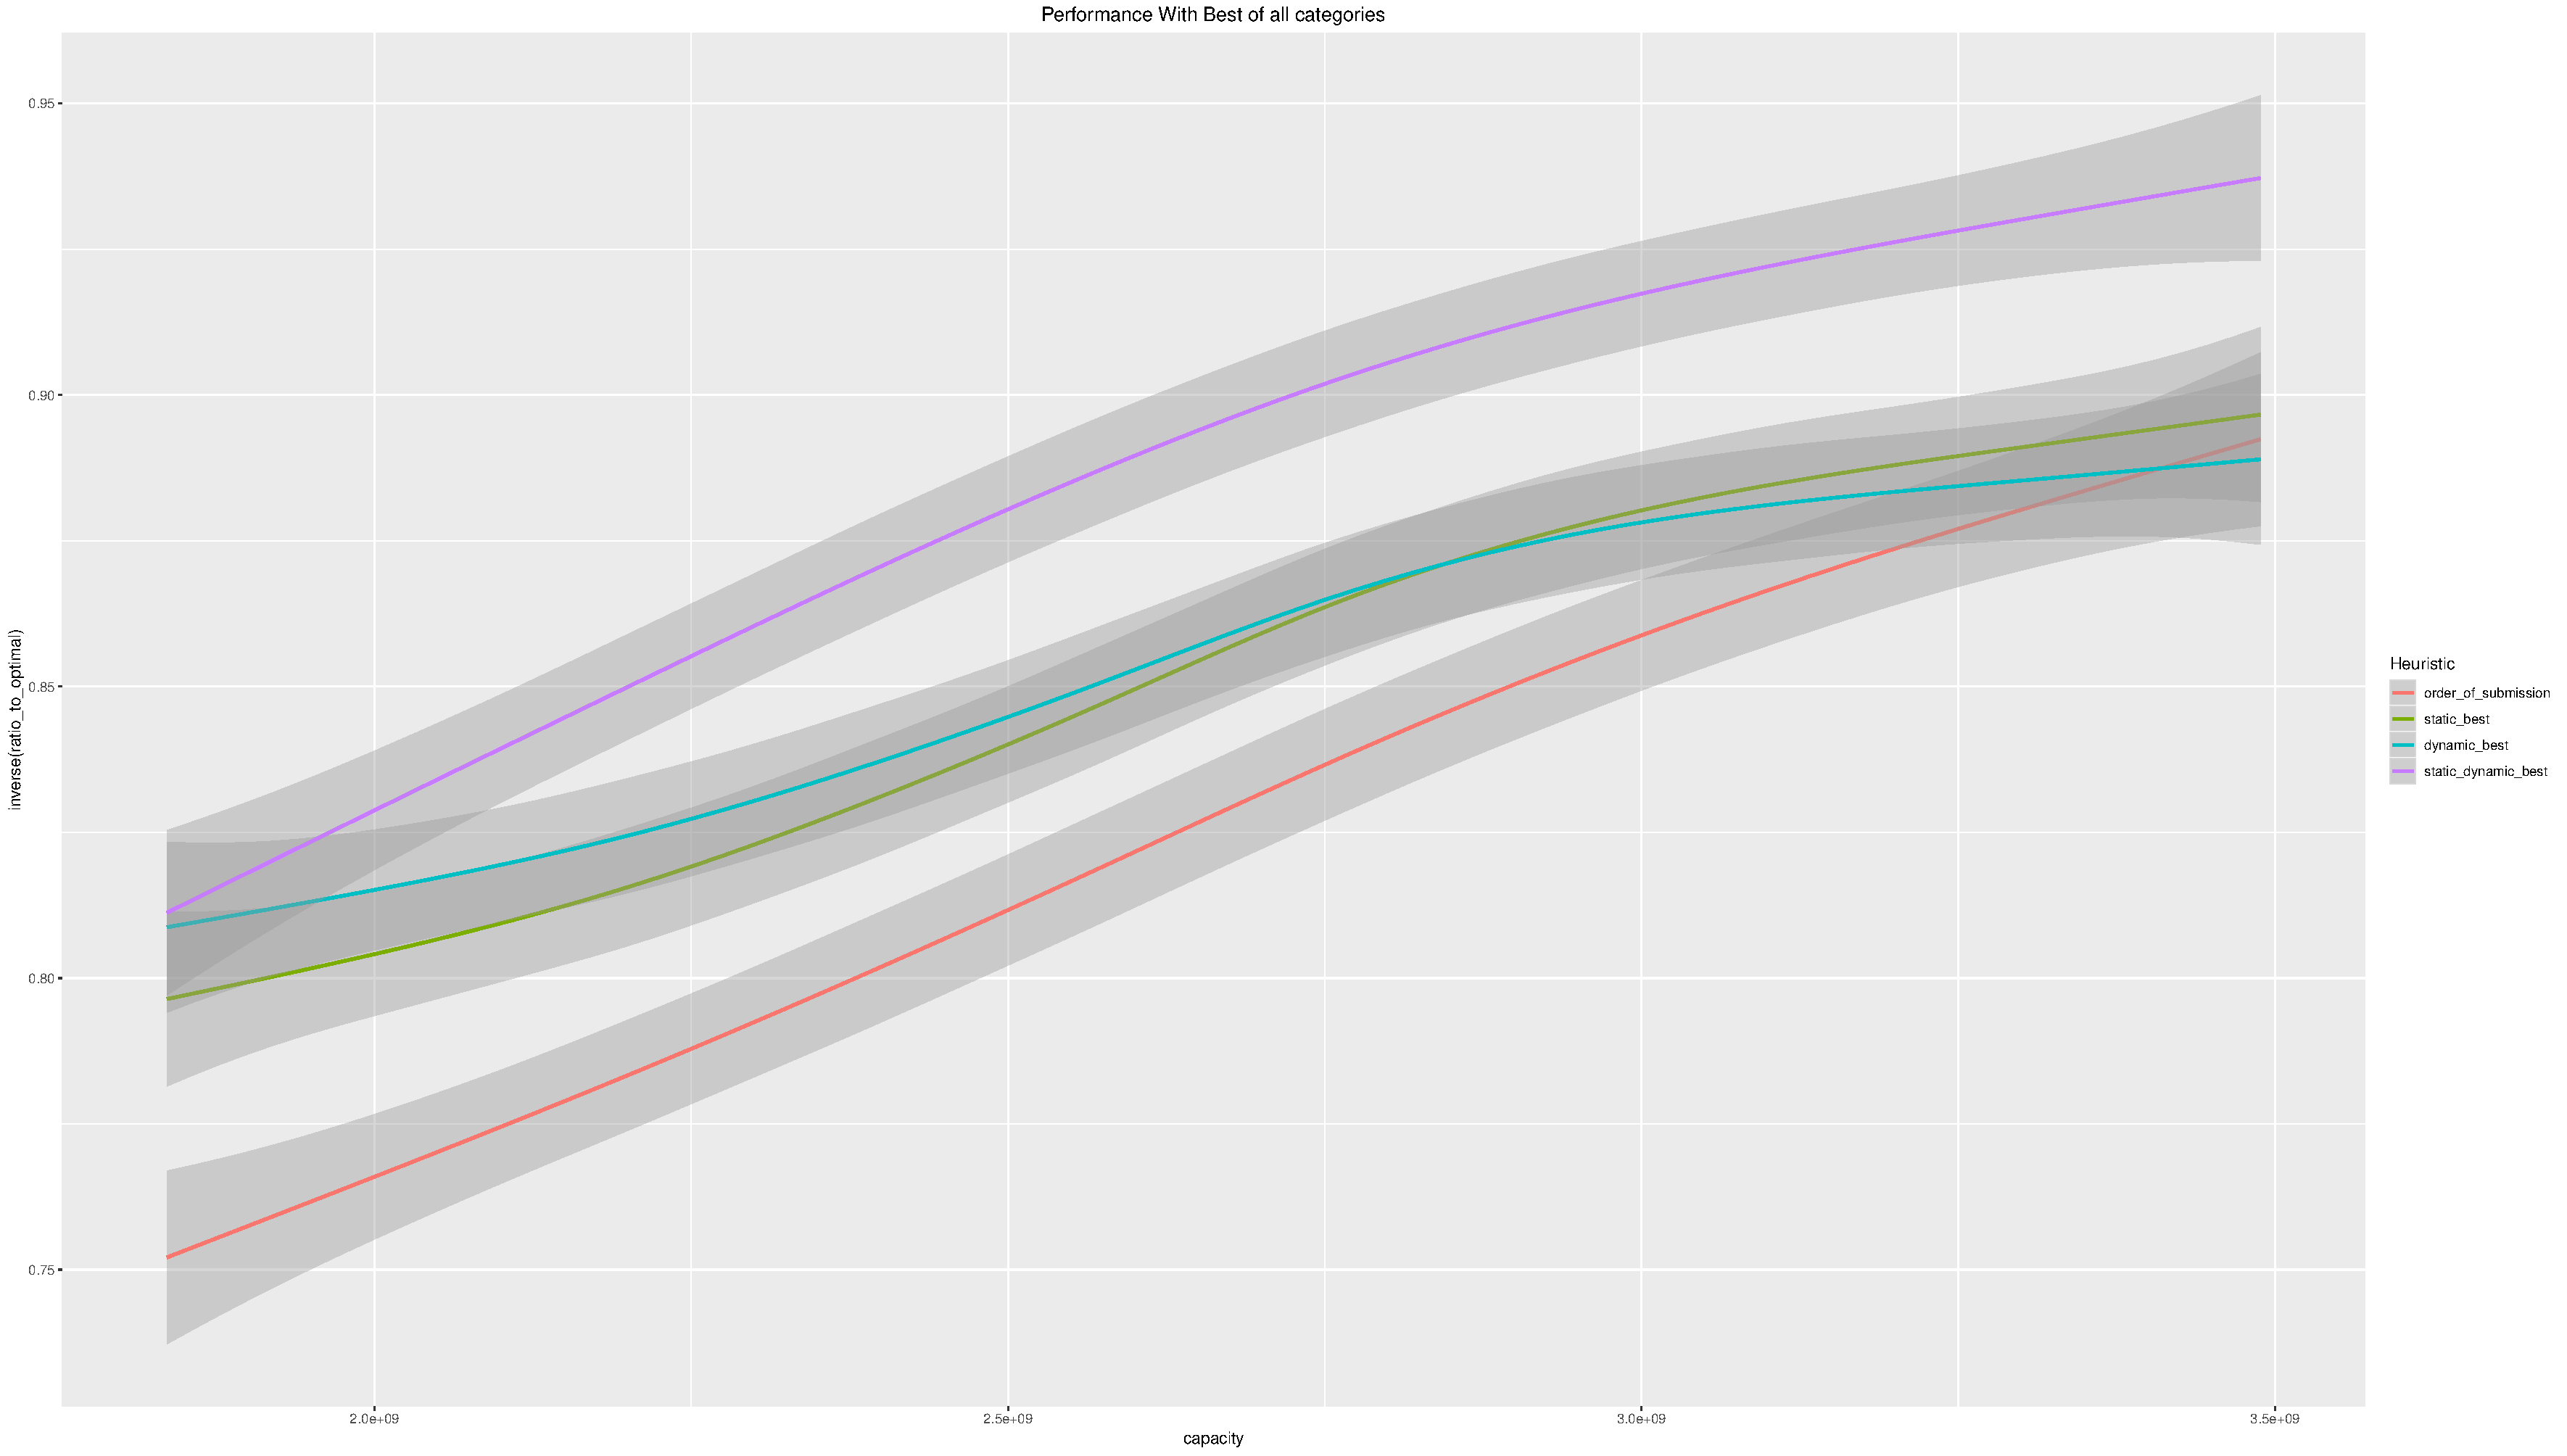
\includegraphics[scale=0.25]{../ExperimentalResults/inverse_ratio_to_optimal_ccsd-best.pdf}
	\caption{Comparision of best variants of all categories for CCSD.}
	\label{fig:ratio_to_optimal_best_ccsd}
	\end{figure}

Figure~\ref{fig:ratio_to_optimal_best_ccsd} shows that best variants of dynamic and static+dynamic strategies achieve similar performance at minimum memory capacity $m_c$. But as memory capacity increases hterogeneity allows static+dynamic strategies to take advantage of static knowledge to get maximum overlap and dynamic correction to select another task in case of memory capacity limitation. Static strategies also start performing better at the end, which indicates that this application has potential for significant communication-computation overlap and pure dynamic strategies are unable to take scheduling decision based on this information.

\subsection{HF and CCSD Characteristics}


  
\begin{figure}[htb]
	\centering
	\begin{subfigure}{.5\textwidth}
		\centering
		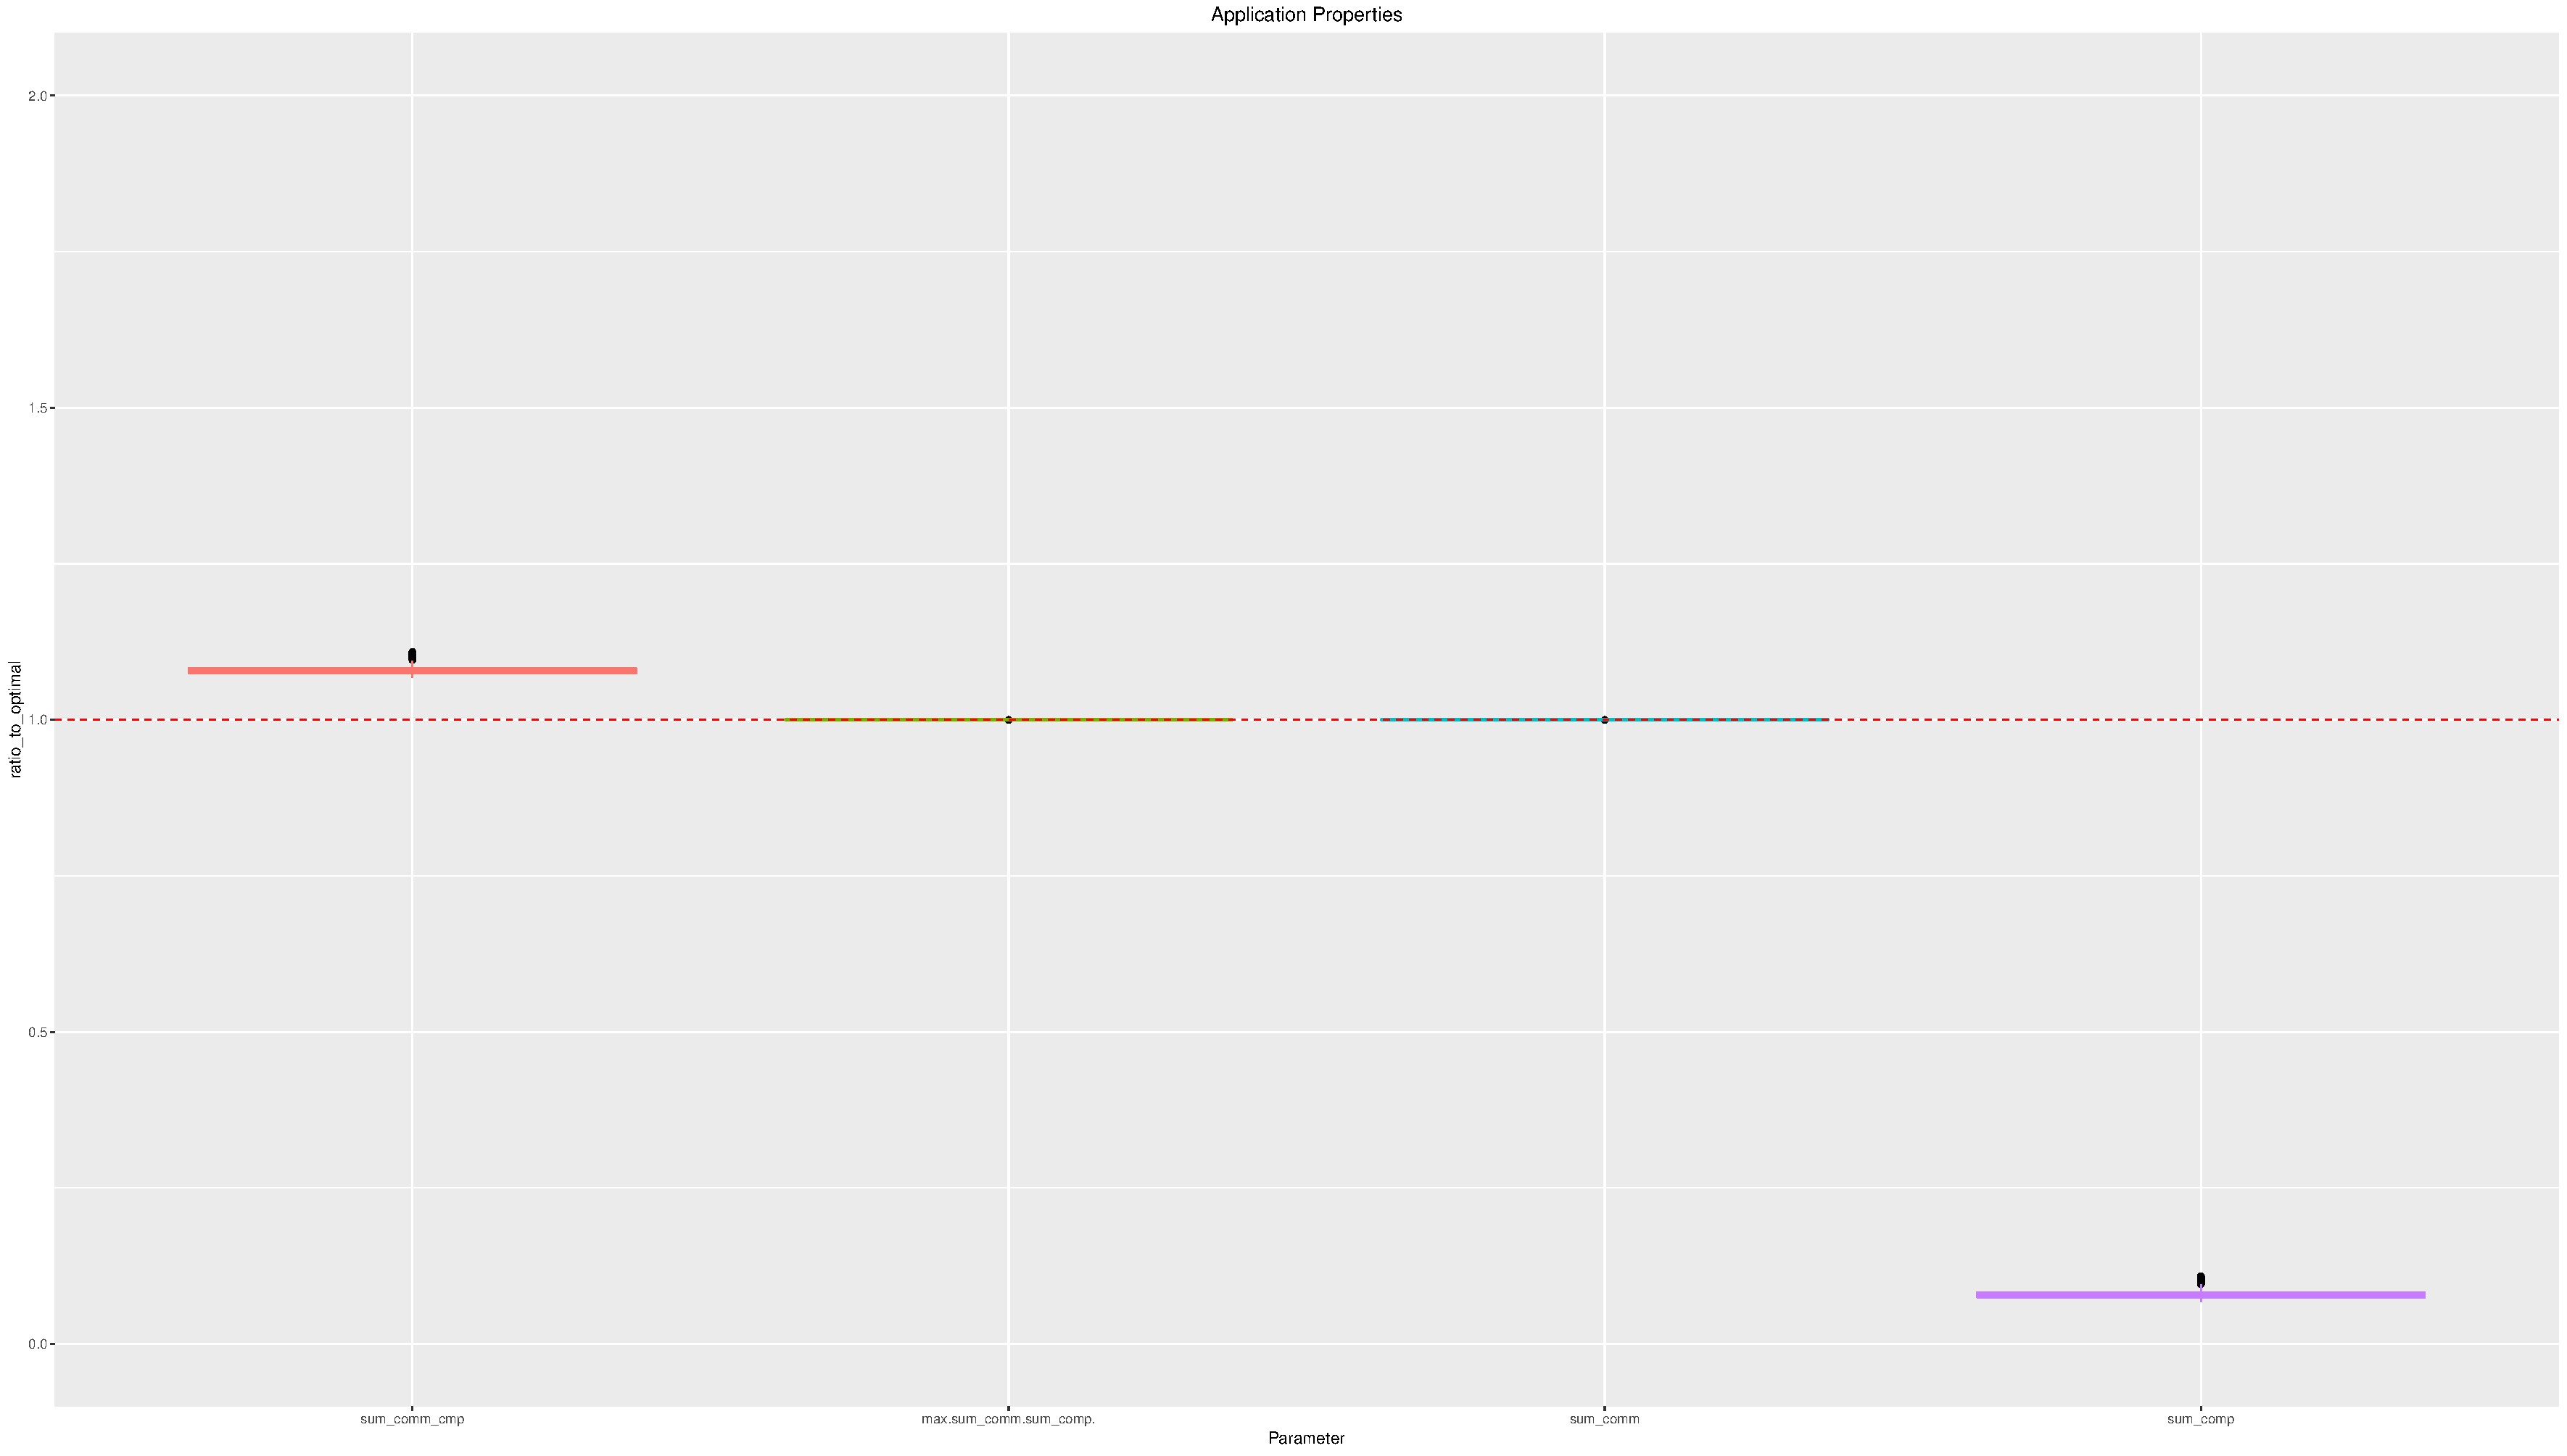
\includegraphics[width=.95\linewidth]{../ExperimentalResults/application_properties_hf.pdf}
		\caption{HF workloads}
		\label{fig:hfProperties}
	\end{subfigure}%
	\begin{subfigure}{.5\textwidth}
		\centering
		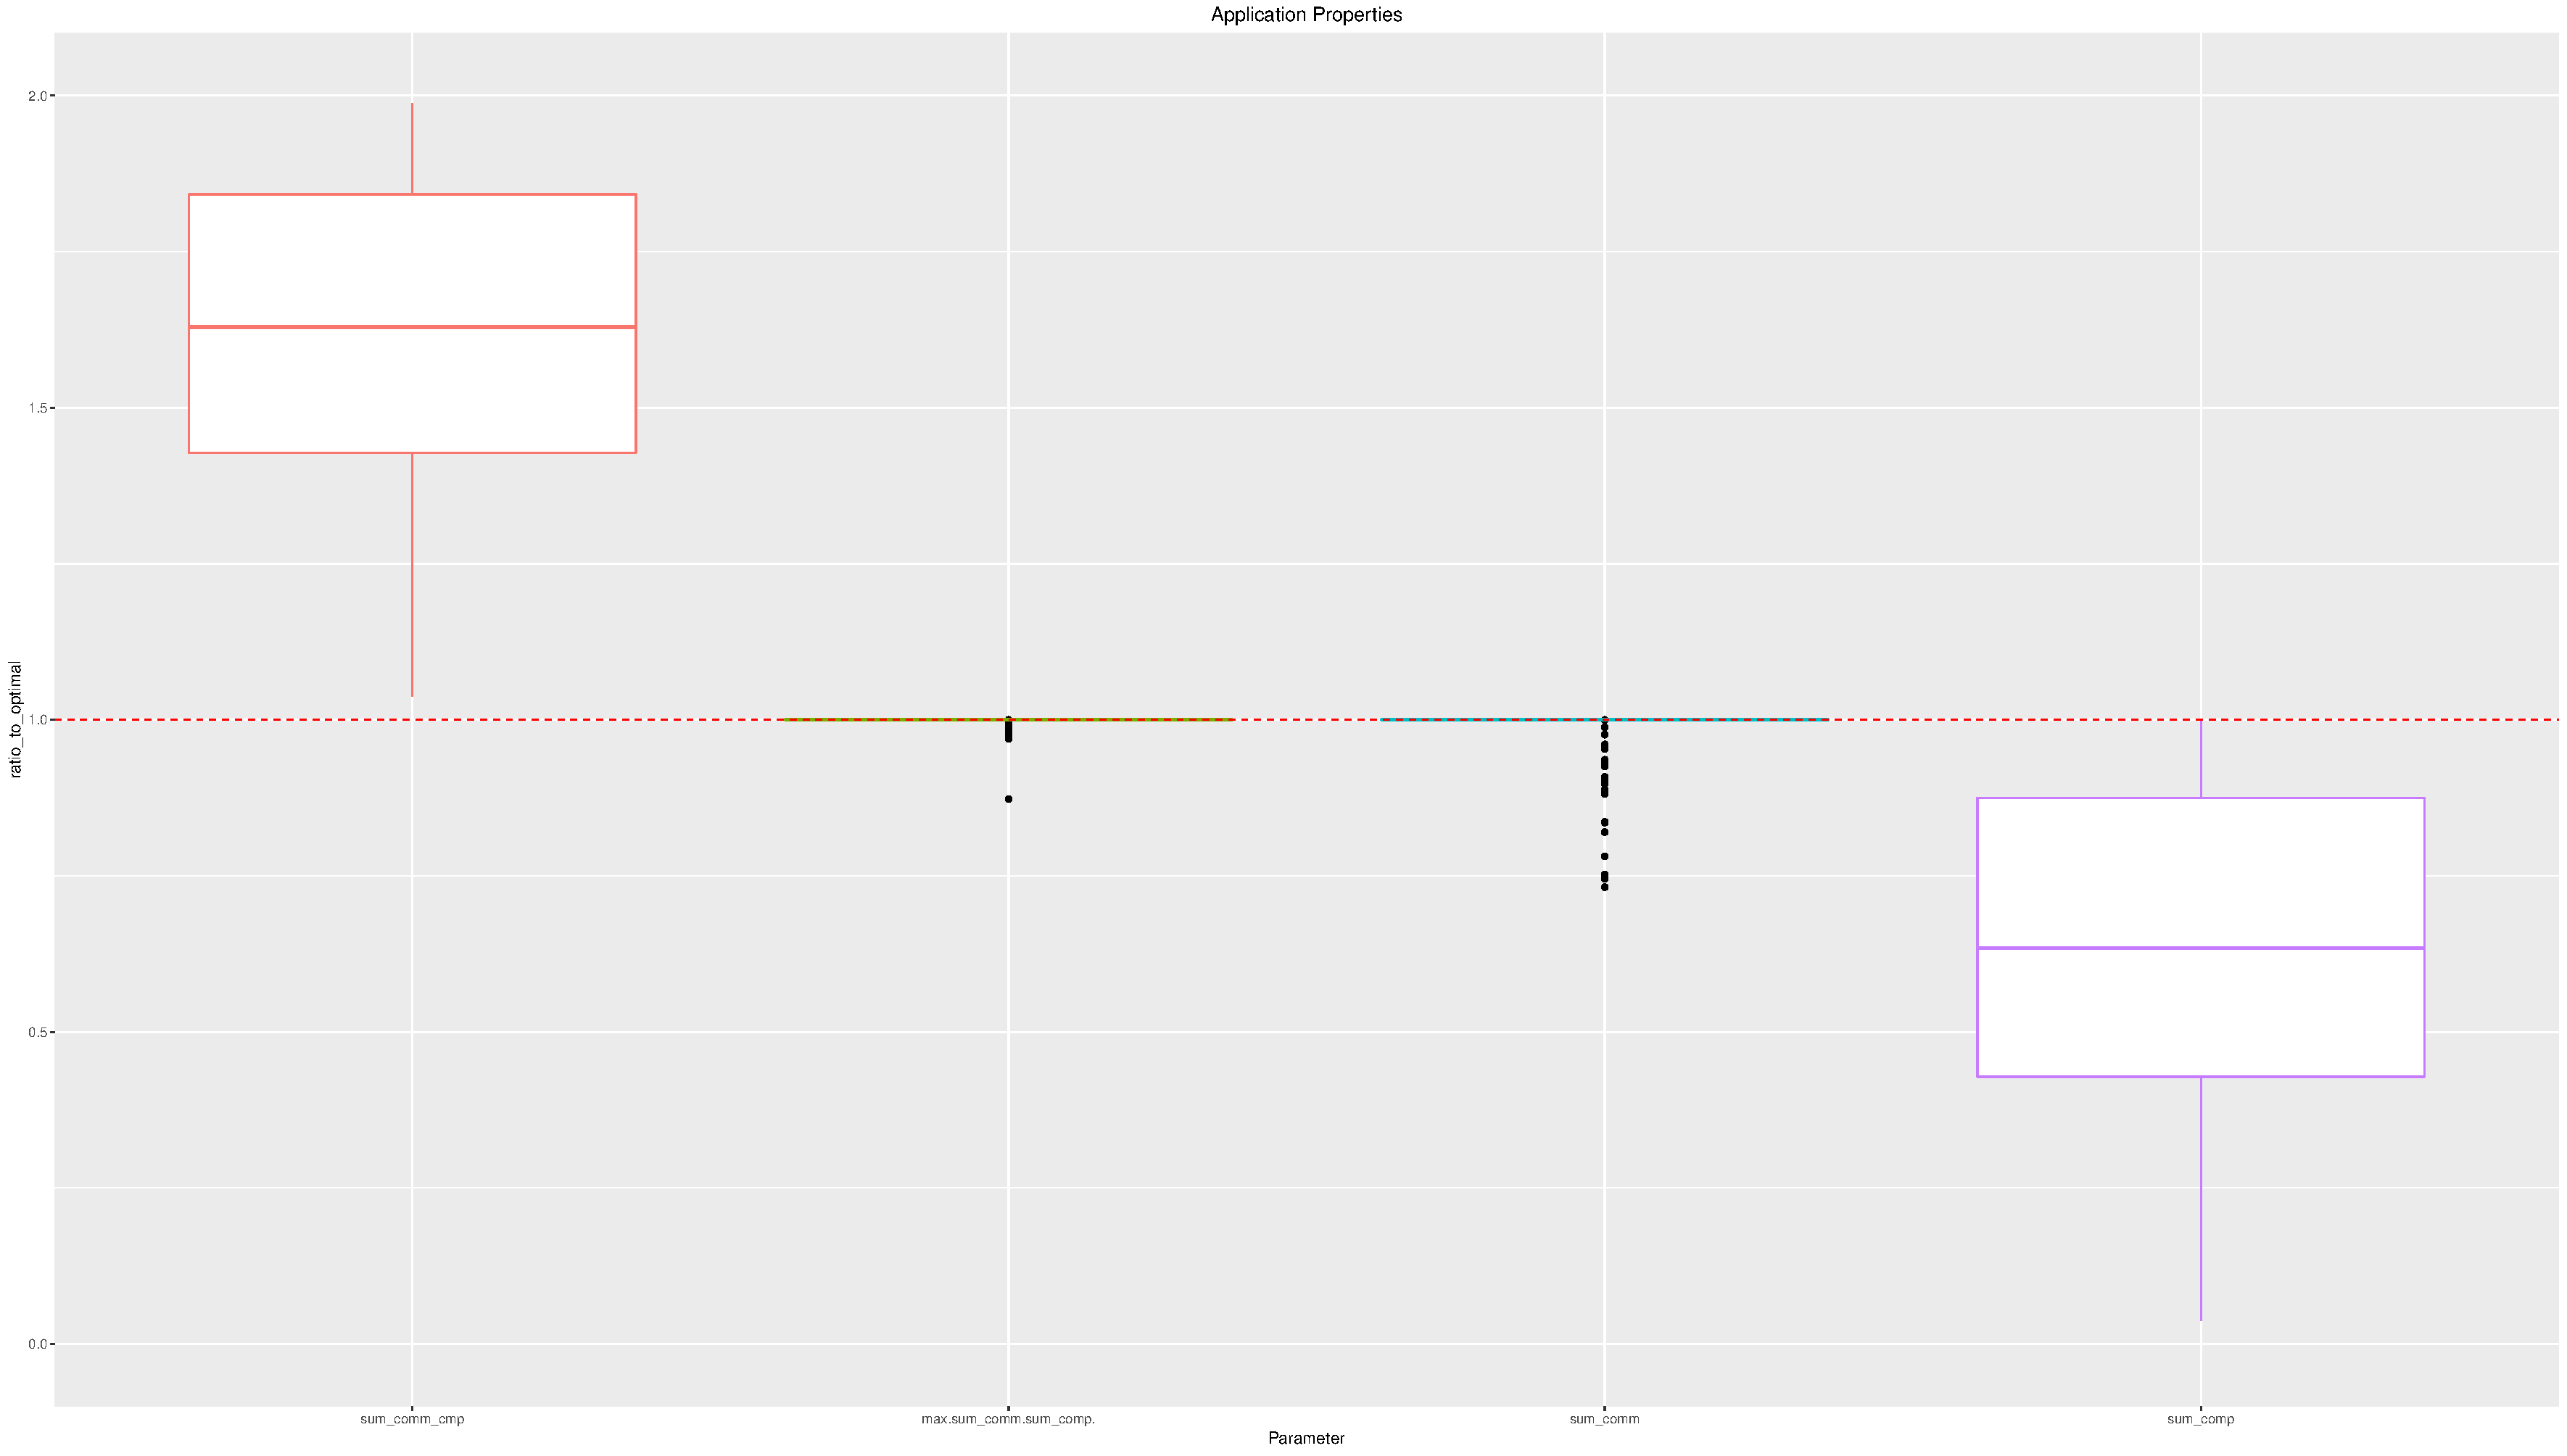
\includegraphics[width=.95\linewidth]{../ExperimentalResults/application_properties_ccsd.pdf}
		\caption{CCSD workloads}
		\label{fig:ccsdProperties}
	\end{subfigure}
	\caption{HF and CCSD tasks characteristics.}
	\label{fig:ApplicationProperties}
\end{figure}

To get more insights into the considered applications, we also look in to their workloads. Figure~\ref{fig:ApplicationProperties} exhibits that HF is a communication intensive application and maximum 20\%  can be expected in the best scenario. While in CCSD , communications and computations are almost evenly distributed and  40-75\% communication-computation overlap is possible.


\subsection{LP Formulation}
%%\todo[inline]{SKumar: LP evaluation and discussion}
%%
%%	\todo[inline]{Skumar: Effect of Random memory with HF or CCSD}
%%	
\subsection{Impact of heterogeneity on different heuristics}

	\begin{figure}[htb]
	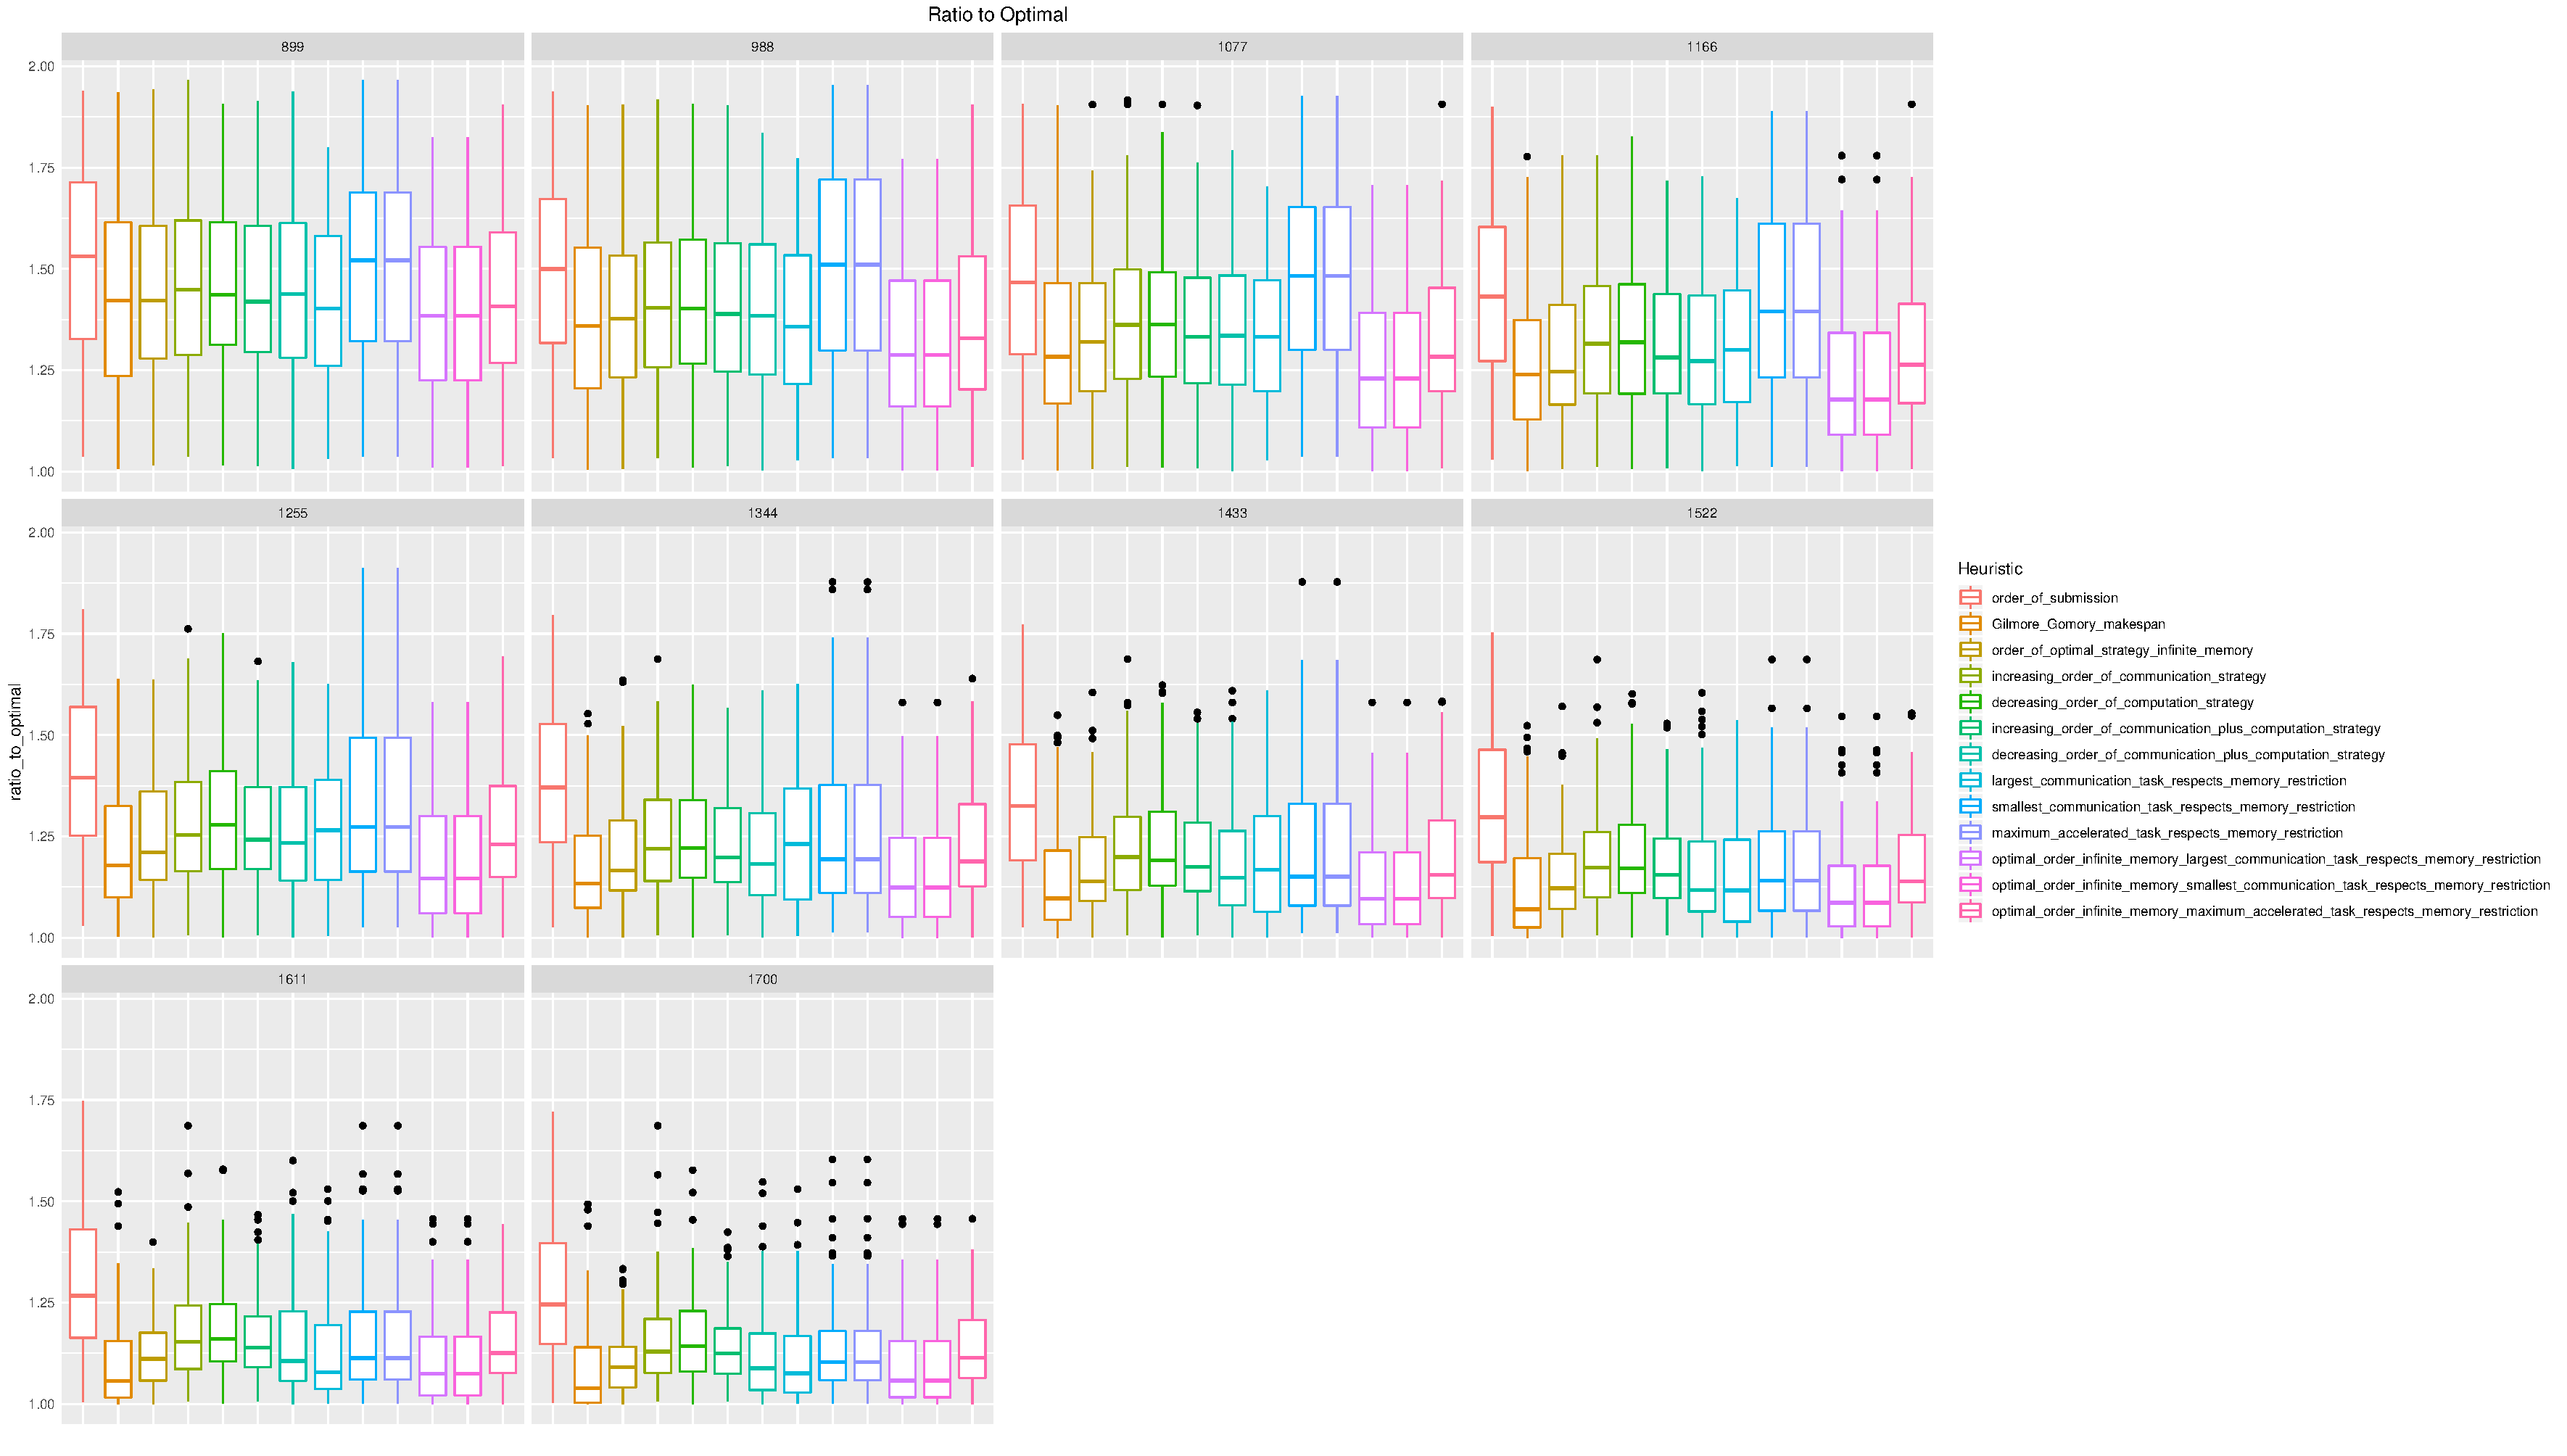
\includegraphics[scale=0.3]{../ExperimentalResults/ccsd-random/ratio_to_optimal_ccsd_random.pdf}
	\caption{Comparison of different heuristics for CCSD with highly heterogeneous tasks.}
	\label{fig:ratio_to_optimal_ccsd_random}
	\end{figure}	


To know the affect of heterogeneity, we set the memory requirement of each task in CCSD trace randomly between 100 to 900 and observe the behavior of different heuristics in  Figure~\ref{fig:ratio_to_optimal_ccsd_random}. This plot also exhibits that static+dynamic variants make good use of static information to maximize communication-computation overlap and dynamic mechanism to minimize the penalty caused by memory capacity limitation. Pure static strategies suffer from memory capacity imitation and pure dynamic strategies are unable to maximize communication-computation overlap.

\subsection{Tasks in Batches}
%%	\begin{figure}[htb]
%%	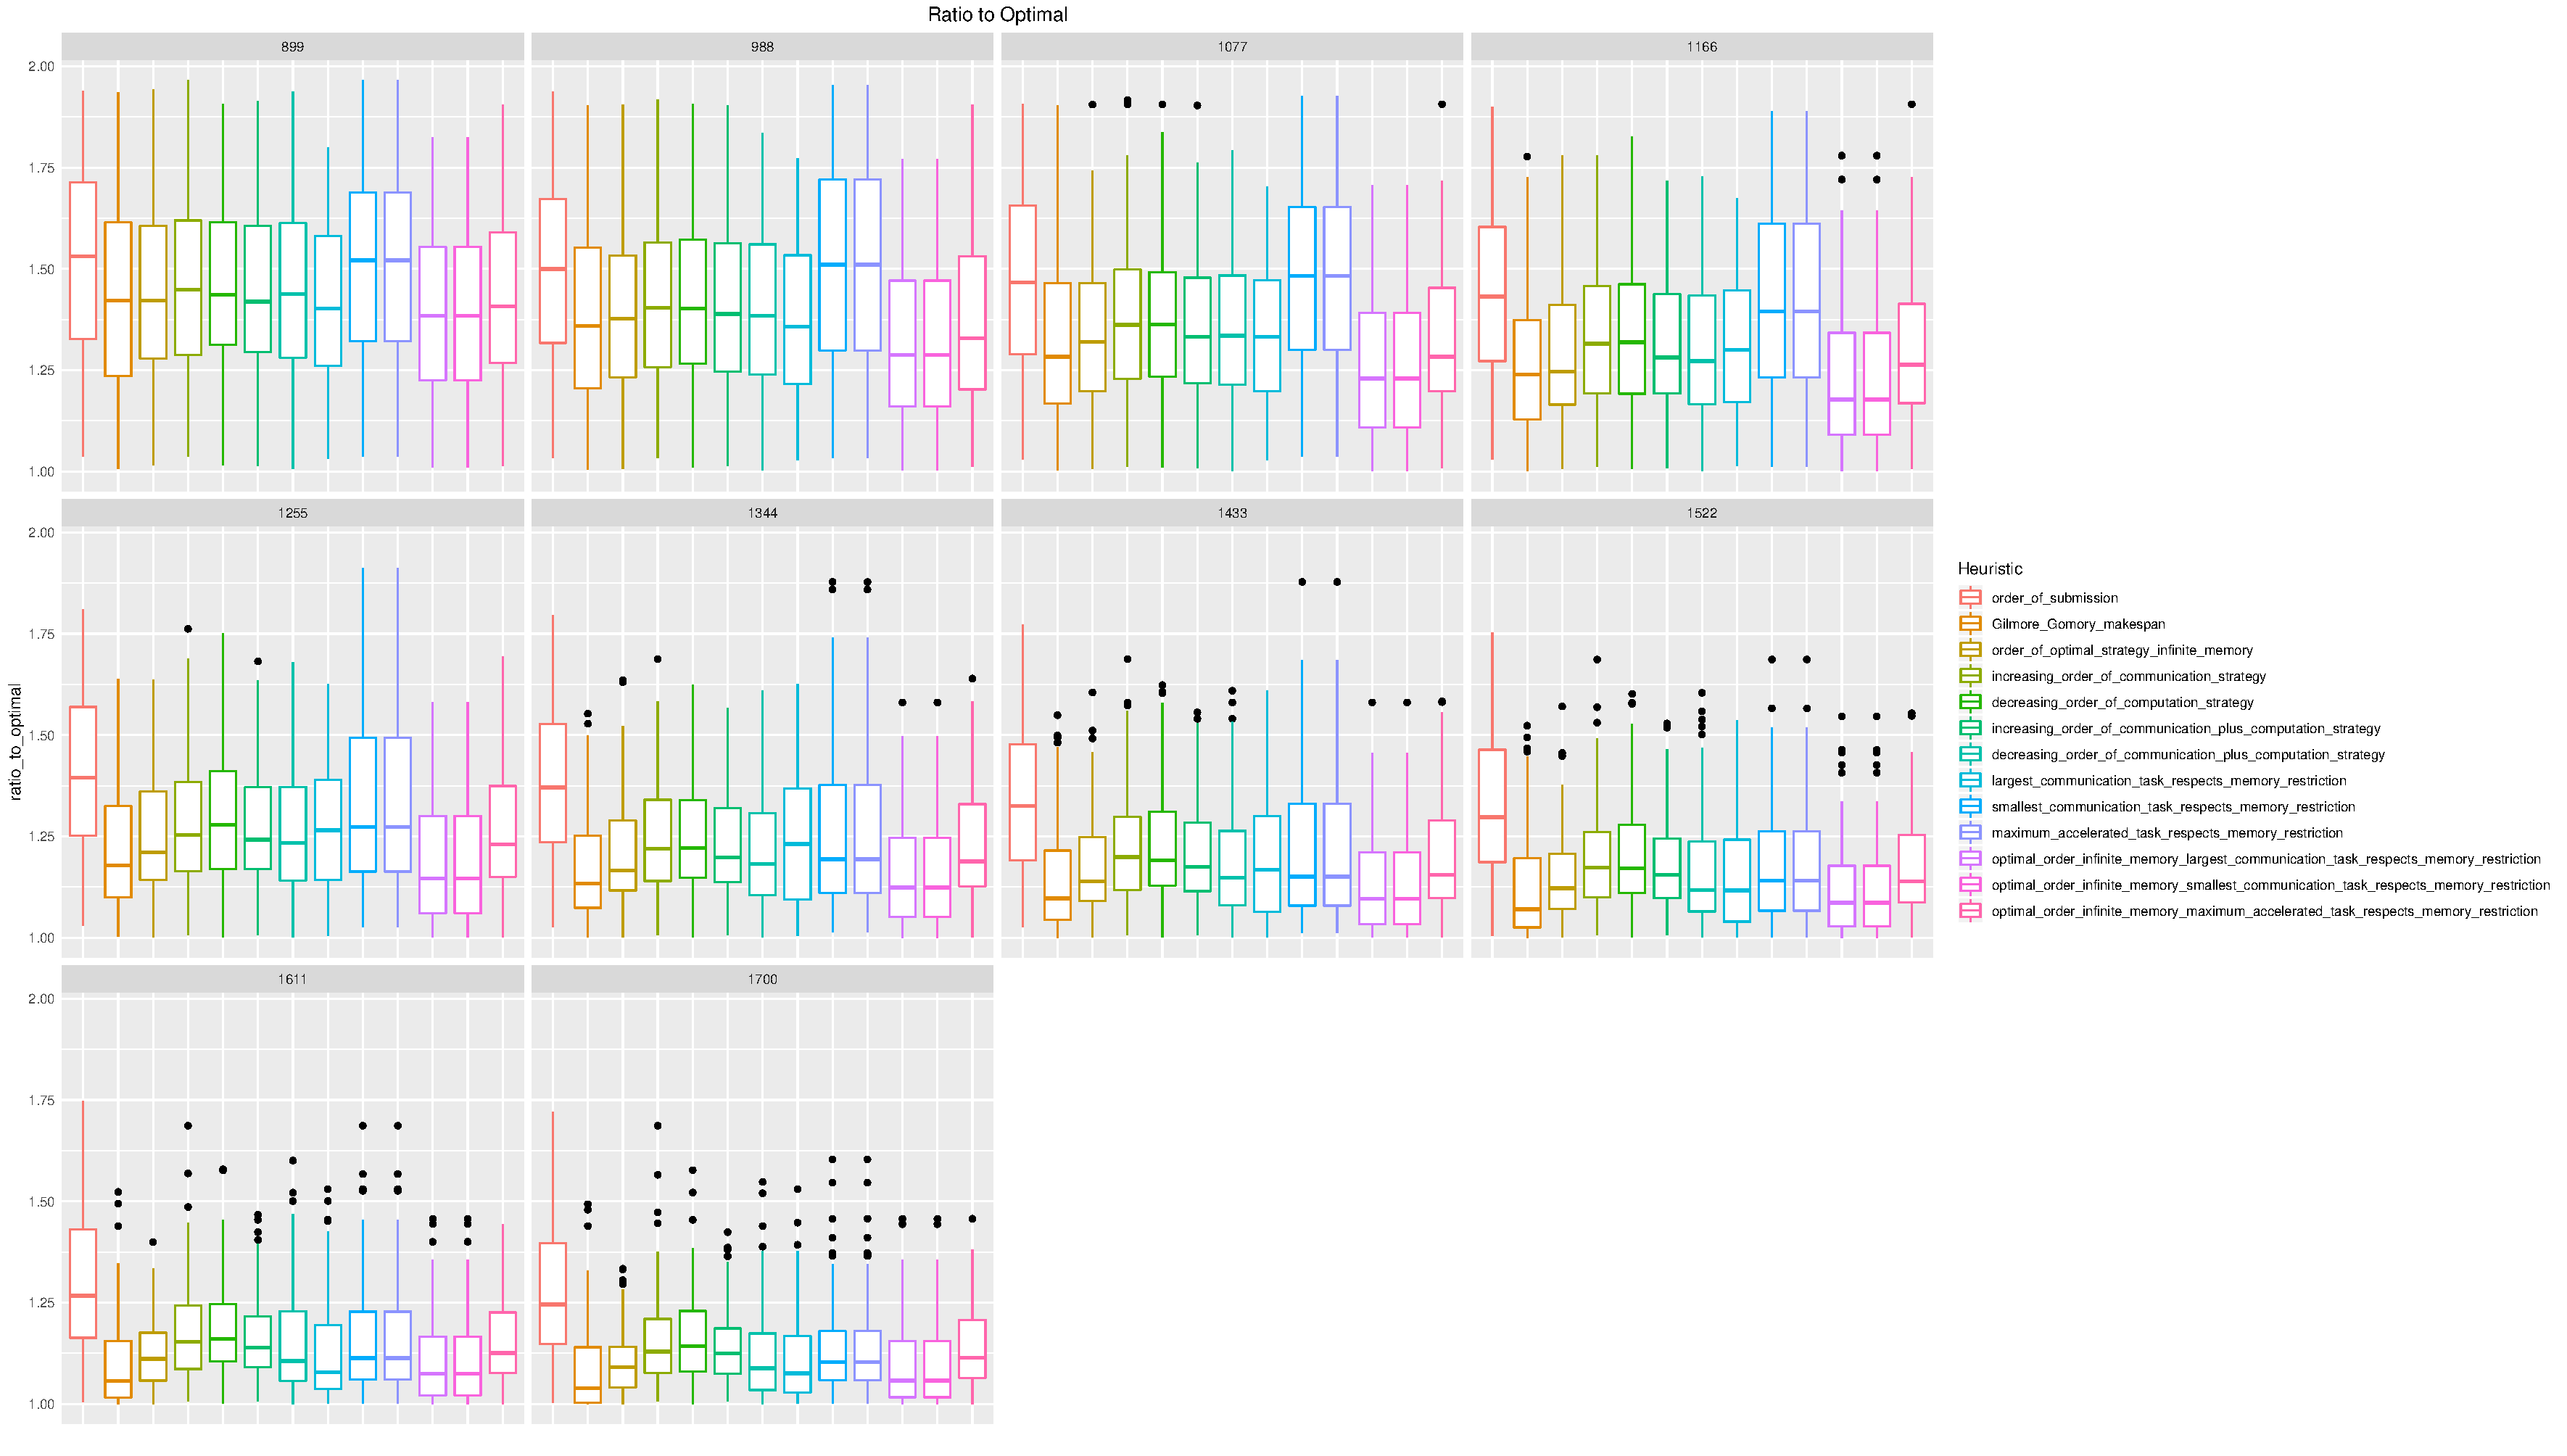
\includegraphics[scale=0.25]{../ExperimentalResults/ccsd-random/ratio_to_optimal_ccsd_random.pdf}
%%	\caption{HF Performance with random memory requirement of a task.}
%%	\label{fig:staticOrderDynamicCorrectionsExample}
%%\end{figure}	

\section{Conclusion and Perspectives}
\begin{itemize}
	\item Evaluated different heuristics
	\item proved NP-complete problem
	\item Plan to implement the best heuristic in a runtime system  for NWChem algorithms and evaluation on Summit supercomputer
\end{itemize}
	
%%	\begin{itemize}
%%		\item Machine description
%%		\item temporary data requirement
%%		\item Description of all kernels (Molecular Chemistry Kernels)
%%		\item Think about results and graphs (Most probably results in $R$ plots)
%%	\end{itemize}

%%%%	\section{First Section}
%%%%	 \subsection{A Subsection Sample} Please note that the
%%%%	first paragraph of a section or subsection is not indented. The first paragraph
%%%%	that follows a table, figure, equation etc. does not need an indent, either.
%%%%	
%%%%	Subsequent paragraphs, however, are indented.
%%%%	
%%%%	\subsubsection{Sample Heading (Third Level)} Only two levels of headings should
%%%%	be numbered. Lower level headings remain unnumbered; they are formatted as
%%%%	run-in headings.
%%%%	
%%%%	\paragraph{Sample Heading (Fourth Level)} The contribution should contain no
%%%%	more than four levels of headings. Table~\ref{tab1} gives a summary of all
%%%%	heading levels.
%%%%	
%%%%	\begin{table} \caption{Table captions should be placed above the
%%%%			tables.}\label{tab1} \begin{tabular}{|l|l|l|} \hline Heading level &  Example &
%%%%			Font size and style\\ \hline Title (centered) &  {\Large\bfseries Lecture
%%%%				Notes} & 14 point, bold\\ 1st-level heading &  {\large\bfseries 1 Introduction}
%%%%			& 12 point, bold\\ 2nd-level heading & {\bfseries 2.1 Printing Area} & 10
%%%%			point, bold\\ 3rd-level heading & {\bfseries Run-in Heading in Bold.} Text
%%%%			follows & 10 point, bold\\ 4th-level heading & {\itshape Lowest Level Heading.}
%%%%			Text follows & 10 point, italic\\ \hline \end{tabular} \end{table}
%%%%	
%%%%	
%%%%	\noindent Displayed equations are centered and set on a separate line.
%%%%	\begin{equation} x + y = z \end{equation} Please try to avoid rasterized images
%%%%	for line-art diagrams and schemas. Whenever possible, use vector graphics
%%%%	instead (see Fig.~\ref{fig1}).
%%%%	
%%%%	\begin{figure} \includegraphics[width=\textwidth]{fig1.eps} \caption{A figure
%%%%			caption is always placed below the illustration. Please note that short
%%%%			captions are centered, while long ones are justified by the macro package
%%%%			automatically.} \label{fig1} \end{figure}
%%%%	
%%%%	\begin{theorem} This is a sample theorem. The run-in heading is set in bold,
%%%%		while the following text appears in italics. Definitions, lemmas, propositions,
%%%%		and corollaries are styled the same way. \end{theorem} %
%%%%	% the environments 'definition', 'lemma', 'proposition', 'corollary',
%%%%	% 'remark', and 'example' are defined in the LLNCS documentclass as well.
%%%%	%
%%%%	\begin{proof} Proofs, examples, and remarks have the initial word in italics,
%%%%		while the following text appears in normal font. \end{proof} For citations of
%%%%	references, we prefer the use of square brackets and consecutive numbers.
%%%%	Citations using labels or the author/year convention are also acceptable. The
%%%%	following bibliography provides a sample reference list with entries for
%%%%	journal articles~\cite{ref_article1}, an LNCS chapter~\cite{ref_lncs1}, a
%%%%	book~\cite{ref_book1}, proceedings without editors~\cite{ref_proc1}, and a
%%%%	homepage~\cite{ref_url1}. Multiple citations are grouped
%%%%	\cite{ref_article1,ref_lncs1,ref_book1},
%%%%	\cite{ref_article1,ref_book1,ref_proc1,ref_url1}. %
%%%%	% ---- Bibliography ----
%%%%	%
%%%%	% BibTeX users should specify bibliography style 'splncs04'.
%%%%	% References will then be sorted and formatted in the correct style.
%%%%	%
%%%%	% \bibliographystyle{splncs04}
%%%%	% \bibliography{mybibliography}
%%%%	%
%%%%	\begin{thebibliography}{8} \bibitem{ref_article1} Author, F.: Article title.
%%%%		Journal \textbf{2}(5), 99--110 (2016)
%%%%		
%%%%		\bibitem{ref_lncs1} Author, F., Author, S.: Title of a proceedings paper. In:
%%%%		Editor, F., Editor, S. (eds.) CONFERENCE 2016, LNCS, vol. 9999, pp. 1--13.
%%%%		Springer, Heidelberg (2016). \doi{10.10007/1234567890}
%%%%		
%%%%		\bibitem{ref_book1} Author, F., Author, S., Author, T.: Book title. 2nd edn.
%%%%		Publisher, Location (1999)
%%%%		
%%%%		\bibitem{ref_proc1} Author, A.-B.: Contribution title. In: 9th International
%%%%		Proceedings on Proceedings, pp. 1--2. Publisher, Location (2010)
%%%%		
%%%%		\bibitem{ref_url1} LNCS Homepage, \url{http://www.springer.com/lncs}. Last
%%%%		accessed 4 Oct 2017 \end{thebibliography} 

\bibliographystyle{IEEEtran}
% argument is your BibTeX string definitions and bibliography database(s)
\bibliography{article}

\end{document}
